\documentclass[11pt]{article}

\usepackage[T1]{fontenc}
\usepackage[utf8]{inputenc}
\usepackage[margin=1.02in]{geometry}
\usepackage{amsmath,amssymb,amsthm,mathtools}
\usepackage{booktabs,tabularx,array,multirow}
\usepackage{enumitem}
\usepackage{graphicx}
\usepackage{microtype}
\usepackage{xcolor}
\usepackage{listings}
\usepackage{tikz}
\usetikzlibrary{
  arrows.meta,
  backgrounds,
  calc,
  decorations.pathreplacing,
  fit,
  matrix,
  positioning,
  shapes.geometric
}
\usepackage[colorlinks=true,linkcolor=blue!45!black,
  citecolor=blue!45!black,urlcolor=blue!45!black]{hyperref}
\usepackage{xurl}
\hypersetup{
  pdftitle={Graphs in Motion: Graph Representations, Small-Step GSLTs, and Compositional Cost},
  pdfauthor={Oruzi and Zarathustra Goertzel}
}

\emergencystretch=2em
\setcounter{topnumber}{4}
\setcounter{bottomnumber}{3}
\setcounter{totalnumber}{7}
\renewcommand{\topfraction}{0.92}
\renewcommand{\bottomfraction}{0.82}
\renewcommand{\textfraction}{0.05}
\renewcommand{\floatpagefraction}{0.72}

\newtheorem{theorem}{Theorem}
\newtheorem{proposition}[theorem]{Proposition}
\newtheorem{principle}[theorem]{Design principle}
\newtheorem{definition}[theorem]{Definition}
\newtheorem{example}[theorem]{Example}
\theoremstyle{remark}
\newtheorem{remark}[theorem]{Remark}

\definecolor{opblue}{RGB}{34,91,155}
\definecolor{semgreen}{RGB}{34,126,92}
\definecolor{costviolet}{RGB}{104,69,151}
\definecolor{futureorange}{RGB}{190,101,24}
\definecolor{negred}{RGB}{174,52,62}
\definecolor{inkgray}{RGB}{72,77,82}
\definecolor{papergray}{RGB}{246,247,249}

\tikzset{
  math/.style={draw=semgreen,very thick,fill=semgreen!7,
    rounded corners=2pt,align=center,inner sep=5pt,font=\small},
  op/.style={draw=opblue,very thick,fill=opblue!7,
    rounded corners=2pt,align=center,inner sep=5pt,font=\small},
  cost/.style={draw=costviolet,very thick,fill=costviolet!7,
    rounded corners=2pt,align=center,inner sep=5pt,font=\small},
  syntax/.style={draw=inkgray,thick,fill=papergray,
    rounded corners=2pt,align=center,inner sep=5pt,font=\small},
  future/.style={draw=futureorange,very thick,dashed,fill=futureorange!6,
    rounded corners=2pt,align=center,inner sep=5pt,font=\small},
  negative/.style={draw=negred,very thick,dotted,fill=negred!5,
    rounded corners=2pt,align=center,inner sep=5pt,font=\small},
  opflow/.style={-{Stealth[length=2.5mm]},very thick,draw=opblue},
  semflow/.style={-{Stealth[length=2.5mm]},very thick,draw=semgreen},
  costflow/.style={-{Stealth[length=2.5mm]},very thick,draw=costviolet},
  futureflow/.style={-{Stealth[length=2.5mm]},very thick,dashed,draw=futureorange},
  forgetflow/.style={-{Stealth[length=2.5mm]},thick,dotted,draw=inkgray},
  lab/.style={font=\scriptsize,align=center,text=inkgray,
    fill=white,inner sep=1pt},
  thmlab/.style={font=\scriptsize\itshape,align=center,
    text=semgreen!70!black,fill=white,inner sep=1pt},
  tinybox/.style={draw=inkgray!75,fill=white,rounded corners=1.5pt,
    align=center,inner sep=3pt,font=\scriptsize}
}

\lstdefinestyle{graphlang}{
  basicstyle=\ttfamily\small,
  columns=fullflexible,
  keepspaces=true,
  frame=single,
  rulecolor=\color{inkgray!45},
  backgroundcolor=\color{papergray},
  keywordstyle=\color{opblue!85!black}\bfseries,
  commentstyle=\color{semgreen!70!black},
  showstringspaces=false,
  aboveskip=7pt,
  belowskip=7pt
}

\newcommand{\code}[1]{\texttt{#1}}
\newcommand{\GSLT}{\mathsf{GSLT}}
\newcommand{\SG}{\mathsf{SimpleGraph}}
\newcommand{\denote}[1]{\mathopen{[\![}#1\mathclose{]\!]}}
\newcommand{\Step}{\mathrel{\longrightarrow}}
\newcommand{\Steps}{\mathrel{\longrightarrow^{\!*}}}
\newcommand{\Path}{\mathsf{Path}}
\newcommand{\Fin}{\mathsf{Fin}}
\newcommand{\Resources}{\mathsf{Resources}}
\newcommand{\Prop}{\mathsf{Prop}}
\newcommand{\futuremark}{\textcolor{futureorange}{\textsf{future}}}
\newcommand{\provedmark}{\textcolor{semgreen!75!black}{\textsf{proved}}}
\newcolumntype{Y}{>{\raggedright\arraybackslash}X}

\title{Graphs in Motion\\
\large A Didactic Theory of Graph Representations, Small-Step GSLTs,
and Compositional Cost}
\author{Oru\v{z}i \and Zarathustra Goertzel}
\date{September 2026 --- working draft}

\begin{document}
\maketitle

\begin{abstract}
A finite graph may be stored as an edge list, adjacency matrix, family of
neighbour rows, finite neighbour sets, incidence matrix, or compressed sparse
row structure.  These carriers describe the same mathematical object but have
different query, revision, conversion, and memory behaviour.  We present a
Lean~4 formalization that keeps those claims separate and then reconnects them
compositionally.  The declarative meaning of every simple-graph
representation is a Mathlib \(SG(\Fin n)\).  A representation refinement is
an actual construction together with a commuting theorem.  We distinguish
such extensional refinements from operational algorithms: wrapping an entire
conversion function in one rewrite records an itinerary, but does not expose
the conversion's internal computation.  The first detailed conversion machine
materializes an edge list as an adjacency matrix by consuming one stored edge
occurrence per rewrite.  Its executable step function is exactly equivalent to
its relational semantics, every step preserves an exact completion invariant,
and its terminal matrix is proved equal to the independent refinement.
The same construction is authored as a nonempty sorted \code{LanguageDef}:
its generic executor consumes one edge occurrence per \code{Write} rule and
builds one persistent symmetric-update node, while an independent denotation
commutes with the detailed matrix machine.
The second detailed LanguageDef moves inside graph mathematics itself.  It
executes append, reverse, and homomorphic map on finite-graph walks, one edge
at a time.  Repeated endpoint indices and explicit adjacency queries make
malformed joins and forged non-edges fail closed; proof-relevant executions
terminate at exactly the corresponding Mathlib walk operations with closed
linear step counts.  From this same sorted constructor inventory and guarded
rewrite relation we generate an endpoint-indexed native walk judgment.  Every
Mathlib walk inhabits that judgment, canonical encodings are injective, and
identity, composition, reversal, and homomorphic map form a certified
reachability proof theory whose operations retain exact GSLT executions.
Semantic invariants are characterized as realizations into discrete semantic
GSLTs.  Resource use is additional proof-relevant structure, not something
recoverable from a bare rewrite relation: costed GSLTs form a category, writer
enrichment is functorial, and cost erasure is natural.

The theory includes positive and negative examples for six ordinary graph
representations; exact refinement maps through a canonical matrix waist; the
first occurrence-level conversion GSLT; semantic machines for revision and
querying; a bridge to ordinary Mathlib
matrices; break-even theorems for migration and maintained multi-view
channels; worked query-centric, edge-centric, revision-heavy, and
space-constrained migration decisions; semantic queries for hypergraphs,
enriched metagraphs, and
distinction graphs; and transport of connectedness, bipartiteness, acyclicity,
degree, and Hamiltonicity.  Ore's and Dirac's theorems are proved over
Mathlib's graph semantics and then transported through every representation
conversion.  A work-in-progress appendix marks the later arrows: detailed
matrix-to-row and row-to-CSR machines, walk cancellation and incremental
trail/path admission, the raw-pattern no-junk theorem, an exact executable
syntax and elaborator, certified SAT/DQBF refinement, and a CeTTa runtime
realization.
The result is both a graph library and a worked
example of how a mathematical library can expose operational meaning without
confusing data layout, semantics, provenance, and cost.
\end{abstract}

\paragraph{Status legend.}
Solid blue arrows in the figures are implemented constructions; their labels
distinguish detailed local rewrites from total refinement functions.  No
algorithmic granularity is inferred from colour alone.  Solid green arrows are
proved semantic interpretations or commuting laws; purple arrows carry
selected resource grades.  Orange dashed arrows are deliberately future work.
Red dotted boxes are negative results: they delimit what cannot be
reconstructed or preserved.  This visual distinction is part of the
mathematical claim, not decoration.

\tableofcontents

\section{One graph, many clothes}
\label{sec:many-clothes}

Consider the path \(0--1--2\).  Figure~\ref{fig:many-clothes} gives four of
its concrete forms.  The representations are not equal as data.  They do,
however, denote the same symmetric, irreflexive adjacency relation.  This is
the first distinction on which the development rests:
\[
  \text{concrete carrier} \quad\neq\quad
  \text{mathematical graph denoted by that carrier}.
\]

\begin{figure}[htbp]
\centering
\resizebox{\textwidth}{!}{%
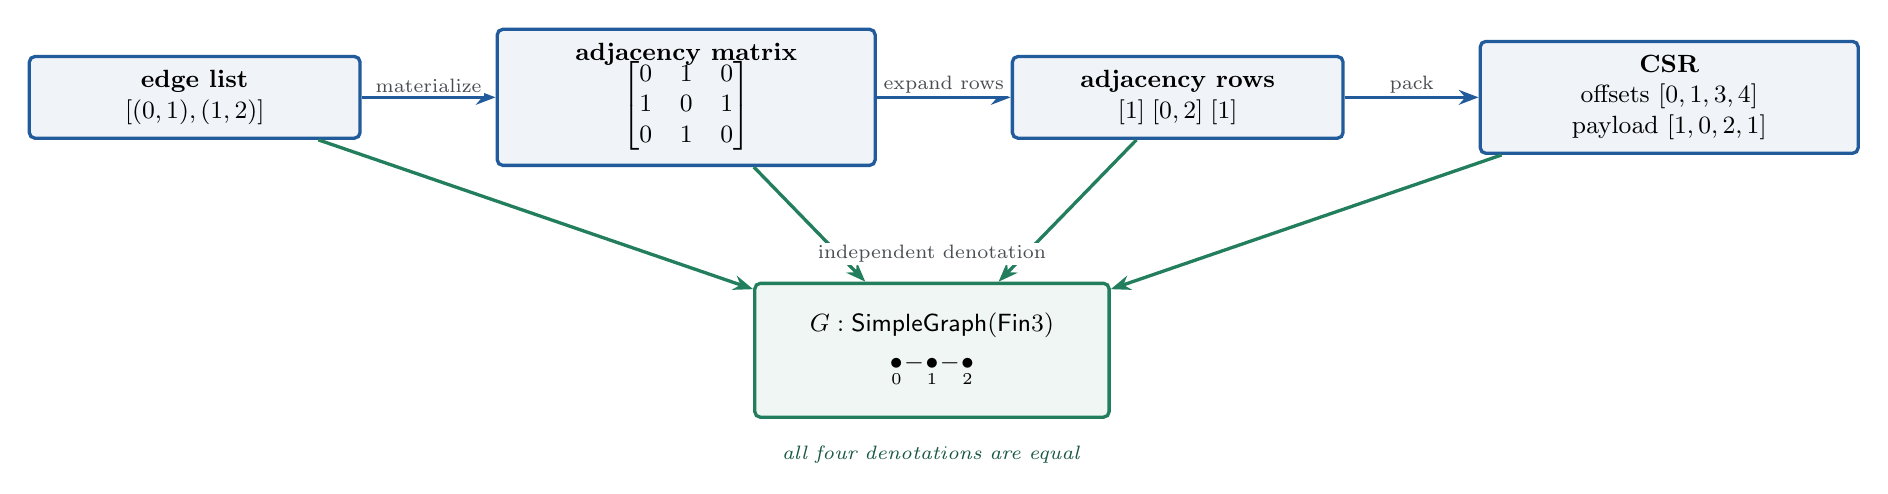
\begin{tikzpicture}[node distance=17mm]
  \node[op,minimum width=42mm] (edges) {
    \textbf{edge list}\\
    \( [(0,1),(1,2)] \)};
  \node[op,right=of edges,minimum width=48mm] (matrix) {
    \textbf{adjacency matrix}\\[-1mm]
    \(\begin{bmatrix}0&1&0\\1&0&1\\0&1&0\end{bmatrix}\)};
  \node[op,right=of matrix,minimum width=42mm] (rows) {
    \textbf{adjacency rows}\\
    \([1]\;[0,2]\;[1]\)};
  \node[op,right=of rows,minimum width=48mm] (csr) {
    \textbf{CSR}\\
    offsets \([0,1,3,4]\)\\
    payload \([1,0,2,1]\)};

  \draw[opflow] (edges) -- node[lab,above] {materialize} (matrix);
  \draw[opflow] (matrix) -- node[lab,above] {expand rows} (rows);
  \draw[opflow] (rows) -- node[lab,above] {pack} (csr);

  \node[math,minimum width=45mm,minimum height=17mm] (meaning)
      at ($(matrix.south)!0.5!(rows.south)+(0,-25mm)$) {
    \(G : \SG(\Fin 3)\)\\[1mm]
    \(\underset{0}{\bullet}\!-\!\underset{1}{\bullet}\!-\!
      \underset{2}{\bullet}\)};

  \foreach \x in {edges,matrix,rows,csr}
    \draw[semflow] (\x) -- (meaning);
  \node[lab,above=2mm of meaning] {independent denotation};
  \node[thmlab,below=3mm of meaning,text width=44mm] {
    all four denotations are equal};
\end{tikzpicture}}
\caption{One graph in several operational forms.  Blue arrows construct new
data.  Green arrows interpret data as a standard mathematical graph.  A
conversion is accepted only after the triangle with the independent meaning
commutes.}
\label{fig:many-clothes}
\end{figure}

The elementary slogan---``one graph, many clothes''---already predicts three
different kinds of motion:
\begin{enumerate}[label=\arabic*.,leftmargin=2.2em]
  \item \emph{conversion} changes the clothes while preserving the graph;
  \item \emph{revision} inserts or erases an edge and therefore changes the
        graph;
  \item \emph{query execution} changes a request into an answer while
        preserving the world being queried and the answer selected from it.
\end{enumerate}
Conflating these motions leads to false invariants, circular semantics, and
misleading cost claims.  Sections~\ref{sec:static}--\ref{sec:query-revision}
separate their mathematical specifications and give small-step GSLTs only
where the local transition structure has actually been defined.

\section{The declarative and operational layers}
\label{sec:layers}

\subsection{The mathematical authority}

For a fixed finite vertex type \(\Fin n\), the declarative authority is
Mathlib's \(\SG(\Fin n)\): a symmetric, irreflexive relation
\cite{mathlib,diestel}.  This choice matters.  The operational development
does not mint a private replacement for ordinary graph theory.  Standard
notions such as connectedness, bipartiteness, acyclicity, neighbourhoods,
degree, walks, and Hamiltonian cycles remain Mathlib predicates and objects.

\subsection{A graph presentation}

A finite graph \emph{presentation} packages just enough to compare concrete
representations:
\[
\begin{aligned}
  P.\mathsf{Carrier} &:\ \mathsf{Type},\\
  P.\mathsf{denote} &:\ P.\mathsf{Carrier}\to\SG(\Fin n),\\
  P.\mathsf{edge} &:\ P.\mathsf{Carrier}\to\Fin n\to\Fin n
      \to \mathsf{Measured}(\mathsf{Bool}),\\
  P.\mathsf{edge\_sound} &:\
      P.\mathsf{edge}(x,u,v).\mathsf{value}=\mathsf{true}
      \ \longleftrightarrow\ P.\mathsf{denote}(x).\mathsf{Adj}(u,v),\\
  P.\mathsf{storageCells} &:\ P.\mathsf{Carrier}\to\mathbb{N}.
\end{aligned}
\]
Here \(\mathsf{Measured}(A)=A\times\mathbb{N}\) records a value and an exact
structural work count.  The count means inspected abstract cells or entries;
it is not asserted to be nanoseconds, cache misses, or machine instructions.

The denotation is chosen independently of the observer.  Thus
\(\mathsf{edge\_sound}\) is evidence rather than a definition by fiat.  This
small directionality choice prevents an implementation bug from becoming
``true'' merely because the implementation returned it.

\subsection{Refinement is a construction plus a theorem}

Given presentations \(P\) and \(Q\), a refinement is
\[
  f : P.\mathsf{Carrier}\to Q.\mathsf{Carrier}
  \qquad\text{with}\qquad
  \forall x,\quad \denote{f(x)}_Q=\denote{x}_P.
\]
The function is load-bearing.  Two separately written implementations that
happen to agree on test outputs are not yet a refinement.  Refinements have
identities and compose in data-flow order, so finite-graph presentations form
a category.  Every refinement also constructs a \emph{channel}
\((x,f(x))\) whose two live views are certified to denote the same graph.

\begin{figure}[htbp]
\centering
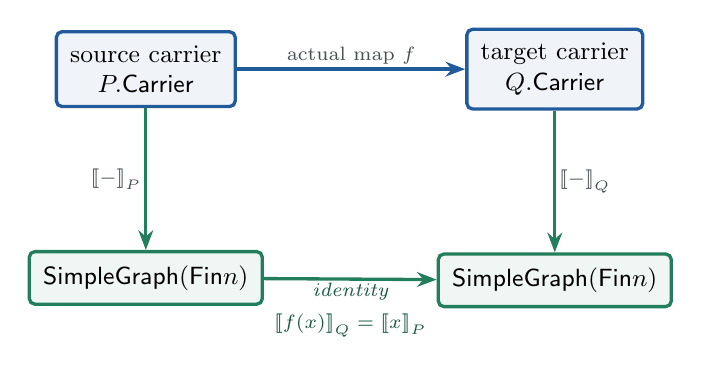
\begin{tikzpicture}[node distance=18mm and 29mm]
  \node[op] (p) {source carrier\\\(P.\mathsf{Carrier}\)};
  \node[op,right=of p] (q) {target carrier\\\(Q.\mathsf{Carrier}\)};
  \node[math,below=of p] (gp) {\(\SG(\Fin n)\)};
  \node[math,below=of q] (gq) {\(\SG(\Fin n)\)};
  \draw[opflow] (p)--node[lab,above]{actual map \(f\)}(q);
  \draw[semflow] (p)--node[lab,left]{\(\denote{-}_P\)}(gp);
  \draw[semflow] (q)--node[lab,right]{\(\denote{-}_Q\)}(gq);
  \draw[semflow] (gp)--node[thmlab,below]{identity}(gq);
  \node[thmlab,below=4mm of $(gp)!0.5!(gq)$] {
    \(\denote{f(x)}_Q=\denote{x}_P\)};
\end{tikzpicture}
\caption{The refinement square.  The upper arrow constructs target data; the
lower comparison says that mathematical graph meaning is unchanged.}
\label{fig:refinement-square}
\end{figure}

\subsection{What a GSLT contributes}

A graph-structured lambda theory is a triple
\(S=(T,E,R)\): terms, an equational setoid, and a rewrite relation respecting
the equations \cite{meredith,turi-plotkin}.  Its proof-relevant paths retain the ordered occurrences of
primitive rewrites.  In this development, a GSLT answers questions that a
static commuting equation cannot:
\begin{itemize}[leftmargin=2em]
  \item Which transformation was actually performed?
  \item In what order were edits and queries consumed?
  \item Which intermediate layouts existed?
  \item How many exposed local rewrite occurrences happened?
  \item What can be reflected from an arbitrary target step or terminal state?
\end{itemize}
The graph meaning may stay fixed even when these operational facts differ.

There is an important granularity condition.  If a rewrite merely applies a
total function that performs the whole conversion, the resulting GSLT records
that the function was invoked and supports path composition, but it does not
yet explain the algorithm inside that function.  We call such an arrow an
\emph{abstract refinement leg}.  A \emph{detailed operational GSLT} instead
exposes the evolving accumulator or worklist, gives local rewrites, relates an
executable successor to those rewrites, and proves that the terminal state
equals an independently specified result.  This paper reserves algorithmic
step and cost claims for the latter.

\section{The finite representation portfolio}
\label{sec:portfolio}

The current portfolio contains six ordinary representations and one enriched
embedding representation.  Table~\ref{tab:portfolio} gives one verified
strength and one verified limitation for each.  The point is not that one
layout is globally best.  The point is that every advantage is indexed by an
observation, and every conversion has a price.

\begin{table}[htbp]
\centering
\small
\renewcommand{\arraystretch}{1.18}
\begin{tabularx}{\textwidth}{@{}>{\bfseries\raggedright\arraybackslash}p{.17\textwidth}
  Y Y@{}}
\toprule
Representation & Positive control & Negative control \\
\midrule
Edge list & Exact authored edge-occurrence enumeration; adjacency is a
left-to-right scan. & An absent edge forces inspection of the entire list.\\
Adjacency matrix & An edge request takes one abstract cell probe and one
query-GSLT step. & Even the empty graph occupies \(n^2\) abstract cells.\\
Adjacency rows & The neighbour list of one vertex is returned exactly. & An
absent neighbour forces a full scan of that vertex's row.\\
Neighbour finsets & Membership and common-neighbour intersection are native
set operations. & Enumeration order and duplicate occurrences are erased.\\
Incidence matrix & A named vertex--edge incidence request takes one abstract
cell probe. & Testing whether two vertices are adjacent may inspect every edge
column.\\
CSR & A vertex row is an exact contiguous slice; storage is linear in offsets
plus payload. & A missing target still forces a full scan of the selected row.\\
Rotation system & The clockwise successor around a vertex is represented
directly. & Forgetting cyclic order is not injective: clockwise and
counterclockwise embeddings may have the same underlying graph.\\
\bottomrule
\end{tabularx}
\caption{Every representation earns a positive and a negative theorem.  Work
counts are structural costs in the selected abstract model, not unqualified
hardware-complexity claims.}
\label{tab:portfolio}
\end{table}

Several qualifications are important.  A finite-set membership request is
one operation in the chosen interface; this does not claim that every concrete
finite-set implementation is constant-time.  Likewise, CSR is cache-friendly
in ordinary implementations, but the formal result here concerns exact slices,
payload sizes, and scans.  A later physical realization must connect those
structural operations to bytes, caches, and wall-clock measurements.

\section{From refinement specifications to a detailed conversion GSLT}
\label{sec:static}

\subsection{The canonical matrix waist}

The library has total refinement functions connecting edge lists, adjacency
matrices, adjacency rows, neighbour finsets, incidence matrices, and CSR.  A
canonical adjacency matrix is their common materialization waist:
\[
  \mathsf{cell}_{x}(u,v)
    := P.\mathsf{edge}(x,u,v).\mathsf{value}.
\]
Soundness of the source edge observer proves symmetry, irreflexivity, and
commutation with \(P.\mathsf{denote}\).  From a matrix the system can build
rows, neighbour finsets, a serialized edge list, an incidence matrix, or CSR
(via rows).

These functions are mathematically substantive: each constructs its target
carrier and has a commuting theorem.  The tagged \code{RepresentationGSLT}
records their composition as abstract refinement legs.  Its one-leg rewrites
do \emph{not}, however, expose the loop or accumulator used inside a
conversion.  Consequently the number of those legs is an itinerary length,
not an algorithmic work count.  The distinction is visible in
Figure~\ref{fig:matrix-waist}: only the first materializer currently has a
detailed small-step semantics.

\begin{figure}[htbp]
\centering
\resizebox{.88\textwidth}{!}{%
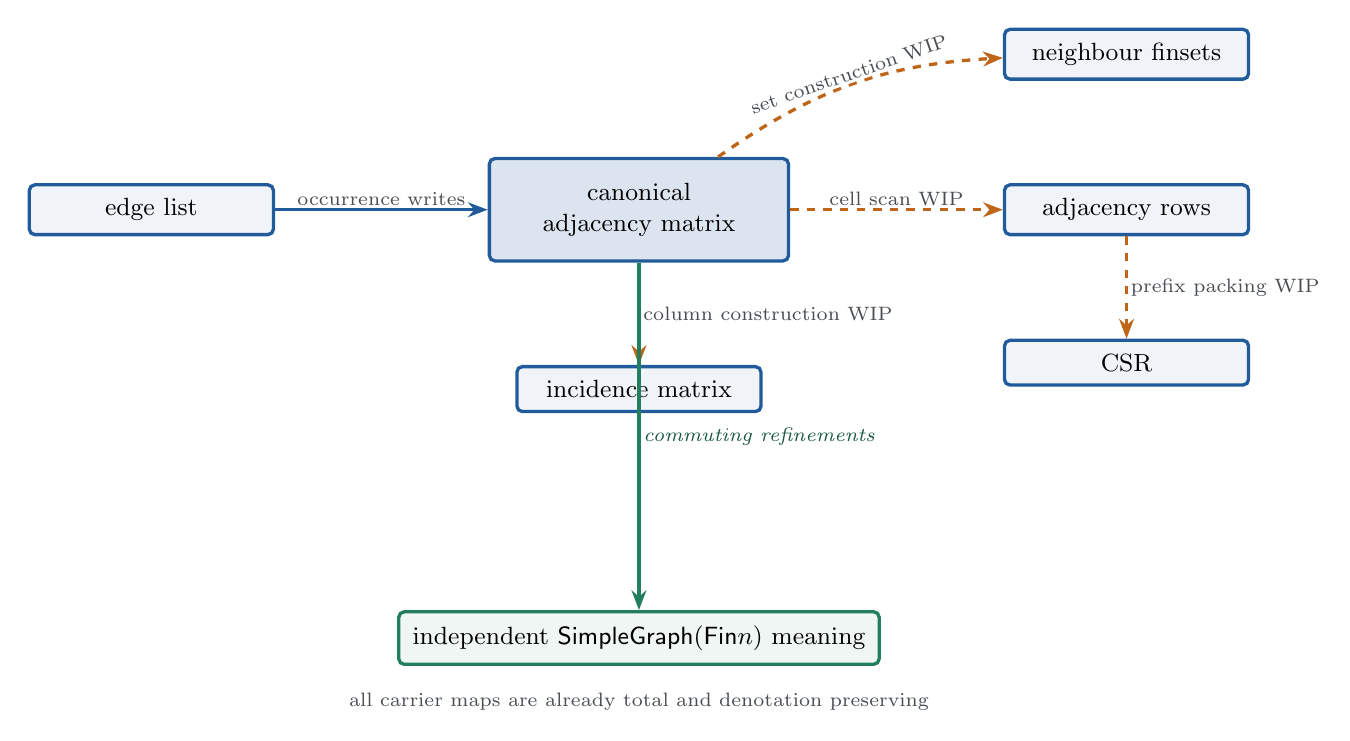
\begin{tikzpicture}[node distance=13mm and 27mm]
  \node[op,minimum width=31mm] (el) {edge list};
  \node[op,right=of el,minimum width=38mm,minimum height=13mm,
    fill=opblue!16] (mx) {canonical\\adjacency matrix};
  \node[op,right=of mx,minimum width=31mm] (ar) {adjacency rows};
  \node[op,below=of ar,minimum width=31mm] (csr) {CSR};
  \node[op,above=of ar,minimum width=31mm] (nf) {neighbour finsets};
  \node[op,below=of mx,minimum width=31mm] (im) {incidence matrix};
  \node[math,below=25mm of im] (sg) {independent \(\SG(\Fin n)\) meaning};

  \draw[opflow] (el) -- node[lab,above]{occurrence writes} (mx);
  \draw[futureflow] (mx) -- node[lab,above]{cell scan WIP} (ar);
  \draw[futureflow] (ar) -- node[lab,right]{prefix packing WIP} (csr);
  \draw[futureflow] (mx) to[bend left=16]
    node[lab,above,sloped]{set construction WIP} (nf);
  \draw[futureflow] (mx) -- node[lab,right]{column construction WIP} (im);
  \draw[semflow] (mx) -- node[thmlab,right]{commuting refinements}(sg);
  \node[lab,below=3mm of sg] {all carrier maps are already total and denotation preserving};
\end{tikzpicture}}
\caption{The matrix is a useful refinement waist, not the definition of graph
meaning.  All displayed conversions already have denotation-preserving total
functions.  The solid edge-list arrow additionally has a detailed small-step
machine; dashed arrows mark the corresponding operational machines still to
be constructed.}
\label{fig:matrix-waist}
\end{figure}

At the abstract-refinement level, every state reaches its canonical matrix in
at most one leg.  Every target other than CSR is constructed from the matrix
in at most one further leg; CSR uses the row intermediate.  Hence every
supported conversion has an abstract path of at most three legs.  For the path
graph of Figure~\ref{fig:many-clothes}, the itinerary
\[
  \mathsf{edgeList}\ \Step\ \mathsf{matrix}\ \Step\
  \mathsf{rows}\ \Step\ \mathsf{CSR}
\]
has three refinement legs.  No claim about three machine operations follows.

\subsection{Occurrence-by-occurrence edge-list materialization}

The detailed edge-list-to-matrix machine starts with an empty lawful Boolean
matrix and retains the unconsumed authored edge occurrences:
\[
  \mathsf{active}(e_1::\cdots::e_k,M)
  \qquad\text{or}\qquad
  \mathsf{done}(M).
\]
One \code{write} rewrite consumes exactly the head occurrence and replaces
\(M\) by a matrix whose addressed symmetric pair is set to true.  A loop
occurrence performs no update, matching simple-graph denotation.  Duplicate
occurrences remain visible as separate rewrites even though Boolean insertion
is idempotent.  Once the list is empty, one \code{finish} rewrite exposes the
accumulator:
\[
\begin{aligned}
  \mathsf{active}(e::es,M)
    &\Step \mathsf{active}(es,\mathsf{insertOccurrence}(M,e)),\\
  \mathsf{active}([],M)
    &\Step \mathsf{done}(M).
\end{aligned}
\]

This state transition is not only relational.  An executable \code{step?}
is proved to return \code{some target} exactly when the rewrite relation holds.
The independently defined completion function folds all remaining occurrences
into the current accumulator.  Every local rewrite preserves that exact
matrix:
\[
  s\Step t \quad\Longrightarrow\quad
  \mathsf{completion}(s)=\mathsf{completion}(t).
\]
For a carrier with \(m\) stored occurrences, the constructed execution path
has exactly \(m+1\) rewrites: one write per occurrence and one finish.  Its
terminal matrix is equal as a carrier, cell for cell, to the pre-existing
extensional refinement \code{Transformations.toMatrix}.  This is the commuting
square required of a genuine algorithmic realization:
\[
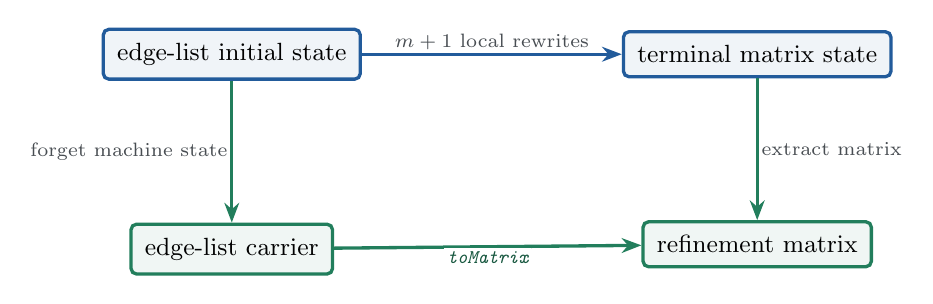
\begin{tikzpicture}[baseline=-2mm,node distance=18mm and 33mm]
  \node[op] (start) {edge-list initial state};
  \node[op,right=of start] (done) {terminal matrix state};
  \node[math,below=of start] (source) {edge-list carrier};
  \node[math,below=of done] (spec) {refinement matrix};
  \draw[opflow] (start)--node[lab,above]{\(m+1\) local rewrites}(done);
  \draw[semflow] (start)--node[lab,left]{forget machine state}(source);
  \draw[semflow] (done)--node[lab,right]{extract matrix}(spec);
  \draw[semflow] (source)--node[thmlab,below]{\code{toMatrix}}(spec);
\end{tikzpicture}
\]

Positive and negative controls make the rules load-bearing.  The two-edge
path takes three rewrites and contains the cells \(0--1\) and \(1--2\); the
non-edge \(0--2\) stays false.  A one-vertex carrier containing only a loop
materializes to the empty matrix.  These examples distinguish occurrence
consumption, no-invention, and loop erasure.

\subsection{The rewrite-bearing LanguageDef}
\label{sec:matrix-langdef}

The detailed state machine also has an authored source in the shared
\code{LanguageDef} format.  It declares five sorts and nine sorted
constructors:
\[
\begin{array}{rcl@{\qquad}rcl}
\mathsf{VertexZero}&:&\mathsf{Vertex} &
\mathsf{VertexSucc}&:&\mathsf{Vertex}\to\mathsf{Vertex}\\
\mathsf{EdgeValue}&:&\mathsf{Vertex}^2\to\mathsf{Edge} &
\mathsf{EdgesNil}&:&\mathsf{Edges}\\
\mathsf{EdgesCons}&:&\mathsf{Edge}\times\mathsf{Edges}\to\mathsf{Edges} &
\mathsf{MatrixEmpty}&:&\mathsf{Matrix}\\
\mathsf{MatrixSetSymmetric}&:&
  \mathsf{Matrix}\times\mathsf{Vertex}^2\to\mathsf{Matrix} &
\mathsf{Active}&:&\mathsf{Edges}\times\mathsf{Matrix}\to\mathsf{State}\\
\mathsf{Done}&:&\mathsf{Matrix}\to\mathsf{State}.&&
\end{array}
\]
The actual definition is assembled as a five-field \code{LanguageDef}; the
only operational authority is its two explicit rewrite rows:
\begin{lstlisting}[style=graphlang,language={}]
def language : LanguageDef :=
  LanguageDef.ofCore "EdgeListToMatrix" types terms []
    [writeRule, finishRule]

Write:
  Active(EdgesCons(EdgeValue(Source, Target), Rest), Matrix)
    ~> Active(Rest,
         MatrixSetSymmetric(Matrix, Source, Target))

Finish:
  Active(EdgesNil(), Matrix) ~> Done(Matrix)
\end{lstlisting}
There is no constructor named \code{convert}, \code{route}, or \code{via},
and neither rewrite invokes a host conversion function.  The generic
\code{LanguageDef} executor matches and instantiates these rows directly.
For every canonical typed state (s), the formalization proves the exact list
equality
\[
  \mathsf{rewriteOnce}(\mathsf{encode}(s))
  = \mathsf{map}(\mathsf{encode},\mathsf{toList}(\mathsf{step?}(s))).
\]
Thus a successful typed action is an actual reduction generated from the
authored definition, and a \code{Done} state has an empty successor list.

The update syntax has an independent interpretation:
\[
\begin{aligned}
\denote{\mathsf{MatrixEmpty}}&=\mathsf{empty},\\
\denote{\mathsf{MatrixSetSymmetric}(M,u,v)}
  &=\mathsf{insertOccurrence}(\denote{M},(u,v)).
\end{aligned}
\]
Every source rewrite commutes with the independently defined detailed
materializer, and folding the generated update expression denotes exactly
\code{Transformations.toMatrix}.  This gives the definition operational
content at the persistent algebraic-update level.  It does not yet claim that
\code{MatrixSetSymmetric} is a mutable row-major implementation; decomposing
that node into address calculation and concrete cell writes remains a lower
physical refinement in Appendix~\ref{app:frontend}.

\subsection{Soundness, exactness, and no invention}

For every abstract refinement leg \(s\Step t\), the theorem
\[
  \denote{s}=\denote{t}
\]
is proved.  It lifts to arbitrary execution paths and, in particular, to the
total abstract conversion path.  Pointwise adjacency therefore satisfies
\[
  \denote{s}.\mathsf{Adj}(u,v)
  \quad\longleftrightarrow\quad
  \denote{\mathsf{convert}(s,L)}.\mathsf{Adj}(u,v).
\]
This is stronger than testing a few outputs: the target cannot invent or erase
an edge.  It is weaker than carrier invertibility, intentionally.  Edge-list
order, duplicate occurrences, matrix layout, and resource history may be lost.
For the detailed materializer, exact endpoint equality strengthens this
denotational theorem and shows that the small-step machine implements the same
carrier function used by the refinement layer.

\section{Walk algebra as an operational LanguageDef}
\label{sec:walk-langdef}

Representation conversion is not the only place where graph mathematics has
useful operational structure.  A Mathlib walk is already an indexed object:
\(\mathsf{Walk}_G(u,v)\) carries its start and end vertices, and every
constructor carries evidence that its next pair is adjacent.  This makes
walk append, reverse, and homomorphic map a particularly clean second
LanguageDef vertical.

The authored language has five sorts,
\(\mathsf{Vertex}\), \(\mathsf{WalkNode}\), \(\mathsf{Walk}\),
\(\mathsf{Frames}\), and \(\mathsf{State}\), and thirteen rewrite rows.  Its
definition is not a wrapper around the three Mathlib functions:
\begin{lstlisting}[style=graphlang,language={}]
def language : LanguageDef :=
  LanguageDef.ofCore "FiniteGraphWalkOperations"
    types terms []
    [ AppendStart, AppendScanCons, AppendScanNil,
      AppendRebuildCons, AppendRebuildNil,
      ReverseStart, ReverseScanCons, ReverseScanNil,
      MapStart, MapScanCons, MapScanNil,
      MapRebuildCons, MapRebuildNil ]

AppendStart:
  AppendRequest(WalkValue(S, M, Left), WalkValue(M, T, Right))
    ~> AppendScan(S, M, T, Left, WalkValue(M, T, Right),
         FramesNil(S))

AppendScanCons [SourceAdjacent(Current, Next)]:
  AppendScan(Current, M, T,
    WalkCons(Current, Next, M, WalkValue(Next, M, Tail)),
    Right, Frames)
      ~> AppendScan(Next, M, T, Tail, Right,
           FramesCons(Next, Current, Frames))

ReverseScanCons [SourceAdjacent(Next, Current)]:
  ReverseScan(Current, T, O,
    WalkCons(Current, Next, T, WalkValue(Next, T, Tail)),
    Accumulator)
      ~> ReverseScan(Next, T, O, Tail,
           prepend(Next, Current, O, Accumulator))

MapScanCons
  [ SourceAdjacent(SourceCurrent, SourceNext),
    MapVertex(SourceNext, MappedNext),
    TargetAdjacent(MappedCurrent, MappedNext) ]:
  MapScan(SourceCurrent, SourceTarget, MappedOrigin,
          MappedCurrent, SourceCons, Frames)
    ~> MapScan(SourceNext, SourceTarget, MappedOrigin,
         MappedNext, SourceTail,
         FramesCons(MappedNext, MappedCurrent, Frames))
\end{lstlisting}
Here \code{prepend} abbreviates the displayed nested
\code{WalkValue}/\code{WalkCons} constructor expression in the source; it is
not an external operation.  The complete definition spells that expression
out.  The scan states accumulate reversed edge frames, and the rebuild rows
pop one frame per step.  Append and map therefore reveal both passes.  Reverse
needs only its scan accumulator.

The relation environment is deliberately small.  It answers one source-edge
query, one target-edge query, or one vertex image under the selected graph
homomorphism.  It never receives or returns a complete walk.  For fully bound
adjacency queries, the formalization proves exact preservation of the binding
fibre.  A vertex-image query introduces exactly its one output binding.  The
three-premise map row then checks the source edge, obtains the next image, and
checks the resulting target edge in that order.

For endpoint-compatible walks \(p : \mathsf{Walk}_G(a,b)\) and
\(q : \mathsf{Walk}_G(b,c)\), and a homomorphism \(f:G\to H\), the generated
proof-relevant paths have the exact endpoints
\[
\begin{array}{rcl}
  \mathsf{AppendRequest}(p,q) &\Step^*&
    \mathsf{WalkDone}(p\mathbin{++}q),\\
  \mathsf{ReverseRequest}(p) &\Step^*&
    \mathsf{WalkDone}(p^{\mathsf{rev}}),\\
  \mathsf{MapRequest}(p) &\Step^*&
    \mathsf{WalkDone}(\mathsf{map}(f,p)).
\end{array}
\]
These endpoints are the ordinary Mathlib operations, not a second private
definition.  If \(\ell(p)\) is the edge length, the retained path lengths are
exactly
\[
  2\ell(p)+3,\qquad \ell(p)+2,\qquad 2\ell(p)+3
\]
for append, reverse, and map respectively.  Thus the cost statement counts
actual authored rewrite occurrences.  It is not a claim about elapsed time or
memory traffic.

The three-vertex path \(0--1--2\) supplies both polarities.  Appending
\(0--1\) to \(1--2\) reaches the two-edge Mathlib walk in five rewrites;
reversing that walk takes four, and mapping it along the identity homomorphism
takes seven.  Conversely, an append request whose first endpoint is \(1\) and
second start is \(2\) has no successor.  A manually forged
\code{WalkCons(0,2,...)} also has no successor because \(0--2\) is not an
edge.  The endpoint repetition and adjacency premise are therefore
load-bearing parts of the semantics.

\section{Native types and reachability proofs}
\label{sec:walk-ntt}

The operational walk language also generates a useful type theory.  This is
not a handwritten predicate renamed ``native.''  Its static component is the
generic executable sort checker instantiated with the complete constructor
table of Section~\ref{sec:walk-langdef}.  Its dynamic component is the
finite-path modality generated from the actual guarded rewrite relation.

For any GSLT \(S\), the formalization constructs the proof-relevant span whose
edges are values of \(S.\mathsf{RewritePath}(s,t)\).  Pullback and dependent
sum along that span yield modalities
\[
  \Diamond^*_{S}P(s)
    \quad\Longleftrightarrow\quad
  \exists t,\;\mathsf{RewritePath}_{S}(s,t)\times P(t),
\]
and, for every \(k\), an exact-length modality \(\Diamond^{k}_{S}\).
Each diamond has its generated right adjoint; the corresponding Galois
connections are proved once in the generic framework rather than separately
for walks.

For a graph \(G\) and vertices \(u,v\), the native walk predicate is the
intersection of three source-derived conditions:
\begin{lstlisting}[style=graphlang,language={}]
NativeWalk(G, u, v, term) :=
  grammarCheck(language, term, Walk)
  and term = WalkValue(u, v, node)
  and DiamondStar(theory(G),
        is WalkDone(WalkValue(v, u, _)),
        ReverseRequest(term))
\end{lstlisting}
The first line comes from the authored constructor signature.  The second is
the fibre of the authored \code{WalkValue} constructor.  The third pulls a
finite-path behavioral type back along the authored
\code{ReverseRequest : Walk -> State} constructor.  It therefore sees every
\code{SourceAdjacent} premise used while scanning the candidate walk.
Mathlib's \code{SimpleGraph.Walk} does not occur in this definition.

The executable checker is itself subject to inversion theorems.  Successful
argument checking consumes exactly one argument per authored parameter; a
checked \code{WalkValue} exposes a checked \code{WalkNode}; and every checked
walk node has outer form exactly \code{WalkNil} or \code{WalkCons}.  These
facts are derived from the constructor table rather than duplicated in a
graph-specific parser.  They isolate the remaining no-junk obligation to
dynamic inversion of the guarded reversal scan.

The present adequacy theorem goes in the semantically important direction:
for every \(p:\mathsf{Walk}_G(u,v)\), its canonical encoding inhabits
\(\mathsf{NativeWalk}(G,u,v)\).  The proof combines a derivation from the
constructor table with the retained reversal path.  Canonical encoding is
injective, so two Mathlib proof objects cannot be collapsed by their native
terms.  The reverse, raw-pattern no-junk theorem---that every term inhabiting
the native type is the encoding of some Mathlib walk---remains open and is
stated as such in Appendix~\ref{app:walk-rewriting}; it is not assumed by the
library organization below.

The distinction between static and dynamic typing is load-bearing.  On the
three-vertex graph \(0--1--2\), a manually formed
\code{WalkCons(0,2,...)} passes the generated constructor-sort checker: its
arguments really do have sorts \code{Vertex}, \code{Vertex}, \code{Vertex},
and \code{Walk}.  It nevertheless fails the native type.  Path decomposition
shows that its reversal request reaches a scanner state, after which no
successor is licensed because \code{SourceAdjacent(2,0)} is false.  Conversely,
an empty walk at vertex \(0\) fails the \(0\to1\) fibre before dynamics are
considered.  Thus constructor sorting, endpoint indexing, and operational
adjacency are three distinct judgments with distinct negative controls.

For library use, a \emph{native reachability proof} pairs a Mathlib walk with
its generated native certificate.  These canonical proof objects support
\[
\begin{aligned}
  \mathsf{id}_u &: u\longrightarrow u,\\
  q\circ p &: u\longrightarrow w,\\
  p^{-1} &: v\longrightarrow u,\\
  f_*p &: f(u)\longrightarrow f(v).
\end{aligned}
\]
Identity and composition satisfy the category laws; reversal is involutive
and reverses composition order; homomorphic map preserves identity and
composition and respects composition of graph homomorphisms.  These are
proved by transporting Mathlib's walk laws through the injective canonical
encoding.  They are also computational statements: composition, inversion,
and map inhabit the exact-length path modalities with the work counts proved
in Section~\ref{sec:walk-langdef}.  Closed walks are already the diagonal
native fibres \(\mathsf{NativeWalk}(G,u,u)\).  Trail and path refinements will
be subtypes only after their own incremental admission machines exist.

\section{What exactly is ``the semantics''?}
\label{sec:semantics}

\subsection{Selected invariants}

For a GSLT \(S\), a semantic invariant with values in \(M\) is an independently
chosen map \(d:S.T\to M\) preserving equations and rewrites.  The library
proves preservation along execution paths and reflexive--transitive execution,
and restricts the operational system to any semantic fibre \(d^{-1}(m)\).

Categorically, this is exact rather than metaphorical:
\begin{theorem}[Invariants as discrete realizations]
For every operational GSLT \(S\) and semantic carrier \(M\), semantic
invariants \(S\to M\) are equivalent to operational realizations
\[
  S\longrightarrow \mathsf{Discrete}(M),
\]
where each source step is sent to the unique zero-length semantic path licensed
by equality of its endpoint denotations.
\end{theorem}

Thus representation conversion is interpreted into a discrete graph GSLT.
This does \emph{not} say that all graph semantics are static.  Revisions need a
non-discrete semantic target, developed in Section~\ref{sec:query-revision}.

\begin{figure}[htbp]
\centering
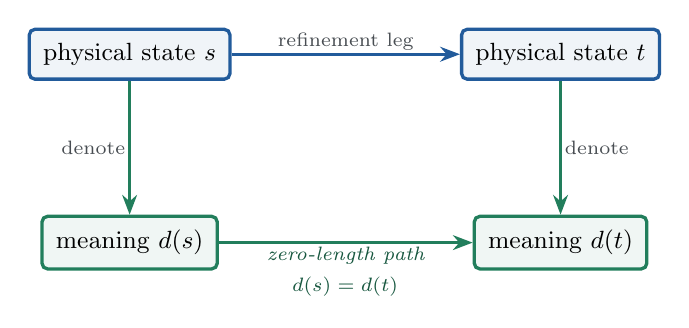
\begin{tikzpicture}[node distance=17mm and 29mm]
  \node[op] (s) {physical state \(s\)};
  \node[op,right=of s] (t) {physical state \(t\)};
  \node[math,below=of s] (ds) {meaning \(d(s)\)};
  \node[math,below=of t] (dt) {meaning \(d(t)\)};
  \draw[opflow] (s)--node[lab,above]{refinement leg}(t);
  \draw[semflow] (s)--node[lab,left]{denote}(ds);
  \draw[semflow] (t)--node[lab,right]{denote}(dt);
  \draw[semflow] (ds)--node[thmlab,below]{zero-length path}(dt);
  \node[thmlab,below=4mm of $(ds)!0.5!(dt)$] {\(d(s)=d(t)\)};
\end{tikzpicture}
\caption{A semantically silent refinement leg.  The source still records a
real construction occurrence and may carry a selected grade; only its graph
meaning is unchanged.  Internal algorithm steps require a detailed machine.}
\label{fig:discrete-realization}
\end{figure}

\subsection{Semantic squares compose}

An operational realization may expand one source step into a finite target
path.  A \emph{denotation square} adds independently selected source and target
meanings and a map between them.  Such squares compose in the same order as
their operational realizations.  This is the reusable answer to
``does the whole pipeline commute?'': each new arrow extends the end-to-end
square rather than merely accumulating pairwise output agreements.

The formalization also proves two useful negative controls:
\begin{itemize}[leftmargin=2em]
  \item stage or layout name is not invariant under representation conversion;
  \item request/answer phase is not invariant under query execution.
\end{itemize}
The surrounding mathematical theory must say which observation is semantic.
A GSLT does not arbitrarily decree that every state field is meaning.

\section{Three motions that must not be conflated}
\label{sec:three-motions}

Figure~\ref{fig:three-motions} is the conceptual centre of the paper.

\begin{figure}[htbp]
\centering
\resizebox{\textwidth}{!}{%
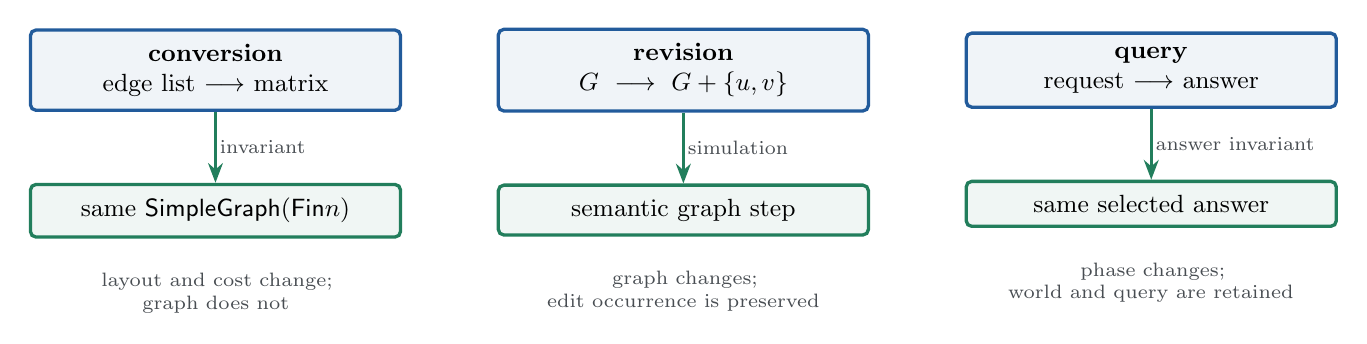
\begin{tikzpicture}[node distance=9mm]
  \node[op,minimum width=47mm] (conv) {
    \textbf{conversion}\\
    edge list \(\Step\) matrix};
  \node[math,below=of conv,minimum width=47mm] (convm) {
    same \(\SG(\Fin n)\)};
  \draw[semflow] (conv)--node[lab,right]{invariant}(convm);

  \node[op,right=12mm of conv,minimum width=47mm] (rev) {
    \textbf{revision}\\
    \(G\ \Step\ G+\{u,v\}\)};
  \node[math,below=of rev,minimum width=47mm] (revm) {
    semantic graph step};
  \draw[semflow] (rev)--node[lab,right]{simulation}(revm);

  \node[op,right=12mm of rev,minimum width=47mm] (qry) {
    \textbf{query}\\
    request \(\Step\) answer};
  \node[math,below=of qry,minimum width=47mm] (qrym) {
    same selected answer};
  \draw[semflow] (qry)--node[lab,right]{answer invariant}(qrym);

  \node[lab,below=4mm of convm,text width=47mm] {
    layout and cost change;\\graph does not};
  \node[lab,below=4mm of revm,text width=47mm] {
    graph changes;\\edit occurrence is preserved};
  \node[lab,below=4mm of qrym,text width=47mm] {
    phase changes;\\world and query are retained};
\end{tikzpicture}}
\caption{The three semantic shapes.  Conversion is a realization into a
discrete graph theory; revision maps to a genuine semantic graph step; query
maps to a semantic request/answer step and then to a discrete answer.}
\label{fig:three-motions}
\end{figure}

\section{Semantic query and revision GSLTs}
\label{sec:query-revision}

\subsection{A reusable semantic query machine}

Given an independent observation function
\(o:W\to Q\to A\), the generic semantic query GSLT has states
\[
  \mathsf{request}(w,q)
  \qquad\text{and}\qquad
  \mathsf{answer}(a),
\]
and exactly the step
\[
  \mathsf{request}(w,q)\Step\mathsf{answer}(o(w,q)).
\]
Its terminal theorem states that every reachable normal answer is exactly
\(o(w,q)\); a separate theorem excludes any different answer.  The selected
answer is itself a semantic invariant, hence an operational realization into
the discrete GSLT on \(A\).

For adjacency matrices, hypergraphs, metagraphs, and sampled distinction
graphs, the concrete query GSLT first translates to this semantic machine and
then to a discrete Boolean answer.  The factorization is visible:

\begin{figure}[htbp]
\centering
\resizebox{.96\textwidth}{!}{%
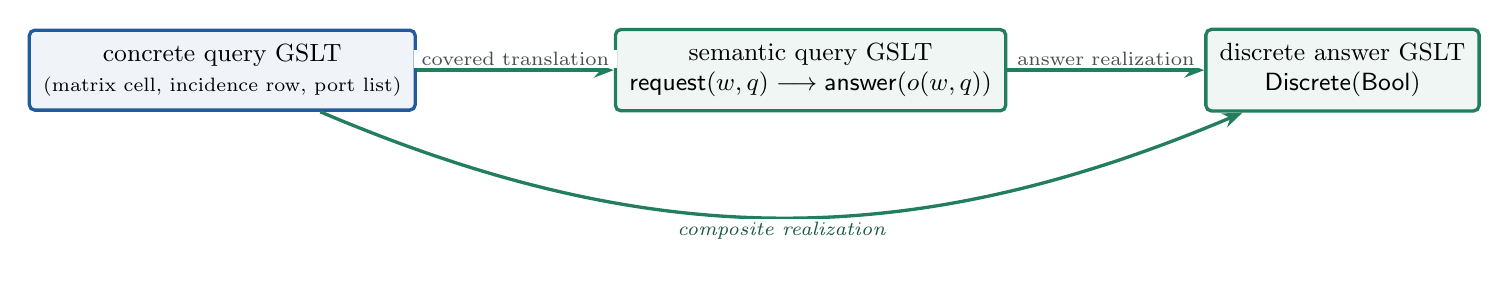
\begin{tikzpicture}[node distance=8mm and 25mm]
  \node[op] (concrete) {concrete query GSLT\\
    \scriptsize(matrix cell, incidence row, port list)};
  \node[math,right=of concrete] (semantic) {semantic query GSLT\\
    \(\mathsf{request}(w,q)\Step\mathsf{answer}(o(w,q))\)};
  \node[math,right=of semantic] (answer) {discrete answer GSLT\\
    \(\mathsf{Discrete}(\mathsf{Bool})\)};
  \draw[semflow] (concrete)--node[lab,above,text width=25mm]{covered translation}(semantic);
  \draw[semflow] (semantic)--node[lab,above,text width=23mm]{answer realization}(answer);
  \draw[semflow,bend right=23] (concrete) to
    node[thmlab,below]{composite realization}(answer);
\end{tikzpicture}}
\caption{Concrete execution does not define truth.  It is translated to an
independent semantic request/answer machine, which in turn conserves the exact
answer.  Covered reverse theorems provide the no-invention boundary.}
\label{fig:query-factorization}
\end{figure}

\subsection{Ordered mixed workloads}

An editable presentation adds a physical edit operation and proves that it
implements an independently defined semantic edit
\(\mathsf{applyMeaning}:\SG(\Fin n)\to\mathsf{EdgeEdit}\to\SG(\Fin n)\).
The mixed workload machine consumes authored edits and queries in order.  Its
state retains the current concrete graph, remaining workload, reverse answer
accumulator, and resource account.  Duplicated queries remain duplicated
answer occurrences.

The independent semantic revision GSLT has no layout or cost field:
\[
\begin{array}{lcl}
\mathsf{active}(G,\,\mathit{work},\,\mathit{answers})
  &\Step&
\mathsf{active}(\mathsf{applyMeaning}(G,e),\,\mathit{rest},\,
  \mathit{answers}),\\[1mm]
\mathsf{active}(G,\,\mathsf{query}(u,v)::\mathit{rest},\,A)
  &\Step&
\mathsf{active}(G,\,\mathit{rest},\,
  \mathsf{decide}(G.\mathsf{Adj}(u,v))::A),\\[1mm]
\mathsf{active}(G,[],A)&\Step&\mathsf{finished}(G,\mathsf{reverse}(A)).
\end{array}
\]
The concrete-to-semantic state map applies the presentation denotation and
drops physical resource/layout fields, but preserves workload order and answer
occurrences.

\begin{figure}[htbp]
\centering
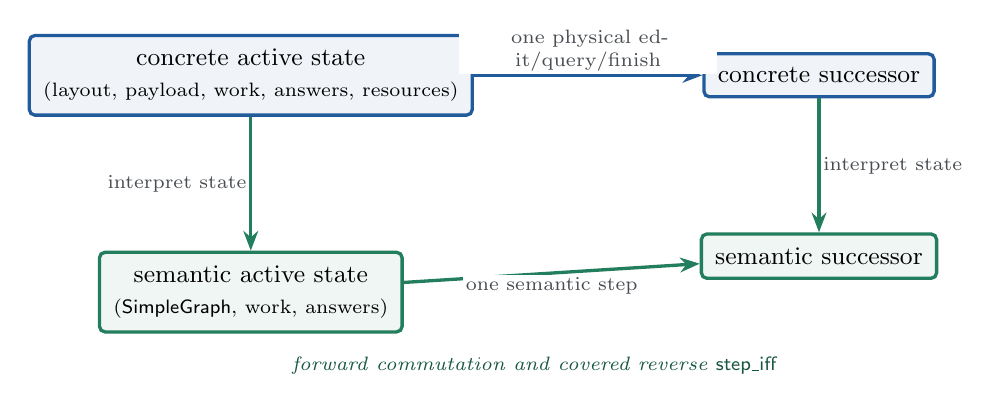
\begin{tikzpicture}[node distance=17mm and 29mm]
  \node[op] (cs) {concrete active state\\
    \scriptsize(layout, payload, work, answers, resources)};
  \node[op,right=of cs] (ct) {concrete successor};
  \node[math,below=of cs] (ss) {semantic active state\\
    \scriptsize(\(\SG\), work, answers)};
  \node[math,below=of ct] (st) {semantic successor};
  \draw[opflow] (cs)--node[lab,above,text width=32mm]{one physical edit/query/finish}(ct);
  \draw[semflow] (cs)--node[lab,left]{interpret state}(ss);
  \draw[semflow] (ct)--node[lab,right]{interpret state}(st);
  \draw[semflow] (ss)--node[lab,below]{one semantic step}(st);
  \node[thmlab,below=6mm of $(ss.south)!0.5!(st.south)$] {
    forward commutation and covered reverse \(\mathsf{step\_iff}\)};
\end{tikzpicture}
\caption{Revision is not forced into a false invariant.  Concrete insertion
maps to semantic insertion, and covered semantic successors reconstruct a
concrete successor.  Full execution agrees with the semantic ordered fold.}
\label{fig:revision-square}
\end{figure}

One-step commutation is strengthened to a covered equivalence: from an
interpreted concrete source, every semantic step is exactly the interpretation
of a concrete successor.  Full execution then yields the same final graph and
ordered answers as semantic execution.  Positive and negative controls show
that insertion really changes adjacency and therefore no graph-denotation
invariant can exist for that step.

\subsection{Physical editing policy}

The adjacency matrix edit changes two symmetric cells and is structurally
in-place in the chosen model.  Other layouts currently use a correct baseline:
canonicalize to a matrix, perform the edit, and materialize the original
layout.  Their positive theorem is semantic correctness; their negative
theorem says that a rebuild with positive target storage is not in-place.
These are intentionally not advertised as optimized update algorithms.  The
interface permits future persistent, differential, and local-update
implementations to compete while preserving the same semantic square.

\section{The ordinary matrix bridge}
\label{sec:matrix}

The graph adjacency-matrix carrier is connected to the standard Mathlib matrix
type \(\mathsf{Matrix}(\Fin n)(\Fin n)\,\mathsf{Bool}\).  Its image is
characterized by
\[
\mathsf{IsSimple}(M) :=
  \bigl(\forall u\,v,\ M_{uv}=M_{vu}\bigr)\ \wedge\
  \bigl(\forall u,\ M_{uu}=\mathsf{false}\bigr).
\]
Conversion to the ordinary matrix is injective; converting back from a matrix
equipped with \(\mathsf{IsSimple}\) is an exact round trip.  Most importantly,
\[
  \denote{A}.\mathsf{Adj}(u,v)
  \quad\longleftrightarrow\quad A_{uv}=\mathsf{true}.
\]

The raw matrix query GSLT has its own request and answer states.  Encoding a
graph-matrix query is answer-blind, and arbitrary-target reflection proves
that a raw matrix step from an encoded source has exactly the encoded graph
successor.  Positive and negative canaries check a genuine path edge and a
false diagonal cell.

\begin{figure}[htbp]
\centering
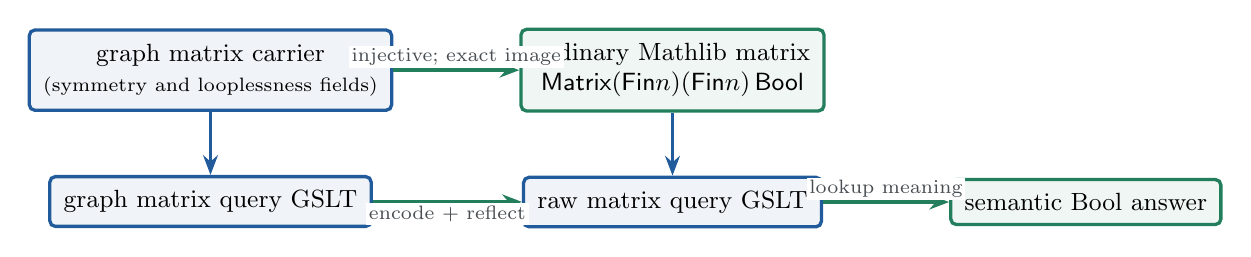
\begin{tikzpicture}[node distance=8mm and 16mm]
  \node[op] (graphm) {graph matrix carrier\\
    \scriptsize(symmetry and looplessness fields)};
  \node[math,right=of graphm] (stdm) {ordinary Mathlib matrix\\
    \(\mathsf{Matrix}(\Fin n)(\Fin n)\,\mathsf{Bool}\)};
  \node[op,below=of graphm] (gquery) {graph matrix query GSLT};
  \node[op,below=of stdm] (mquery) {raw matrix query GSLT};
  \node[math,right=of mquery] (bool) {semantic Bool answer};
  \draw[semflow] (graphm)--node[lab,above]{injective; exact image}(stdm);
  \draw[opflow] (graphm)--(gquery);
  \draw[opflow] (stdm)--(mquery);
  \draw[semflow] (gquery)--node[lab,below]{encode + reflect}(mquery);
  \draw[semflow] (mquery)--node[lab,above]{lookup meaning}(bool);
\end{tikzpicture}
\caption{The matrix representation participates in ordinary matrix
mathematics and in matrix GSLTs.  The graph semantics, matrix semantics, and
query execution agree without identifying their carriers.}
\label{fig:matrix-bridge}
\end{figure}

This bridge is the natural entry point for future matrix-GSLT algorithms:
Boolean matrix multiplication, transitive closure, semiring path problems, or
linear-algebraic graph kernels can state their mathematical correctness over
standard matrices and their operational behavior as GSLT realizations.

\section{Cost is selected structure, not hidden semantics}
\label{sec:cost}

\subsection{A resource monoid}

The graph resource account has five coordinates:
\[
  r=(\mathit{time},\mathit{reads},\mathit{writes},
      \mathit{allocated},\mathit{peakTemporary}).
\]
Sequential composition adds the first four coordinates and takes the maximum
of peak temporary space, reflecting non-overlapping temporary lifetimes:
\[
  (r\mathbin{\star}s).\mathit{peakTemporary}
    =\max(r.\mathit{peakTemporary},s.\mathit{peakTemporary}).
\]
The zero account is a unit and \(\star\) is associative.  Persistent
construction has the abstract peak envelope
\[
  S_{\mathrm{source}}+S_{\mathrm{target}}+S_{\mathrm{temp}},
\]
whereas a destructive lower envelope is
\[
  \max(S_{\mathrm{source}},S_{\mathrm{target}})+S_{\mathrm{temp}}.
\]
The latter is only a lower-envelope model: a concrete algorithm must prove
that it attains it.  Structural in-place execution means zero allocation and
zero temporary cells, not merely low time.

\subsection{Why a bare GSLT has no canonical cost}

A rewrite relation is proposition-valued, and the same local step can
lawfully receive different grades under different physical models.  The
formal negative canary grades one step by one unit in one model and two units
in another.  Therefore there is no canonical cost endofunctor on bare GSLTs.

The correct domain is the category whose objects are pairs
\((S,\gamma)\), where \(S\) is a GSLT and \(\gamma\) is a selected monoidal
grading of its steps.  Morphisms preserve both operational steps and grades.
Writer enrichment is functorial on this category, and erasing the accumulated
writer account is a natural transformation to the underlying operational
theory \cite{moggi}.

\begin{figure}[htbp]
\centering
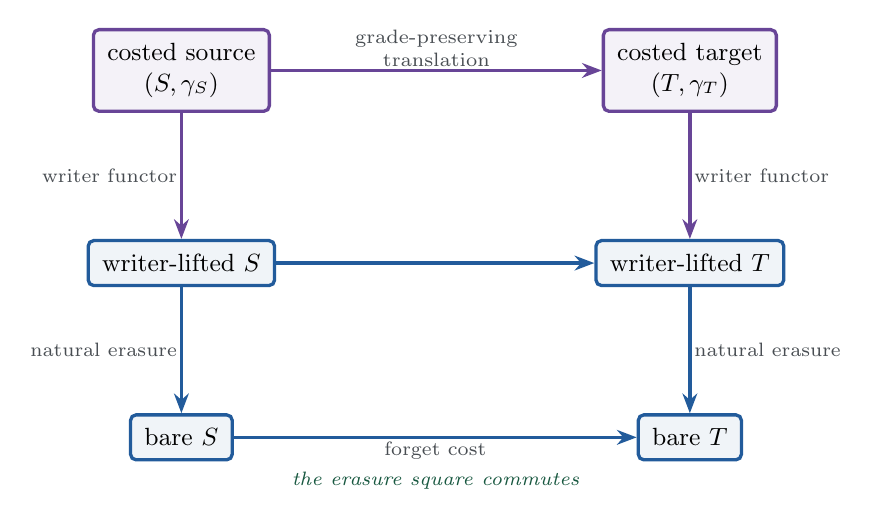
\begin{tikzpicture}[node distance=16mm and 42mm]
  \node[cost] (cs) {costed source\\\((S,\gamma_S)\)};
  \node[cost,right=of cs] (ct) {costed target\\\((T,\gamma_T)\)};
  \node[op,below=of cs] (ws) {writer-lifted \(S\)};
  \node[op,below=of ct] (wt) {writer-lifted \(T\)};
  \node[op,below=of ws] (bs) {bare \(S\)};
  \node[op,below=of wt] (bt) {bare \(T\)};
  \draw[costflow] (cs)--node[lab,above,text width=34mm]{grade-preserving translation}(ct);
  \draw[costflow] (cs)--node[lab,left]{writer functor}(ws);
  \draw[costflow] (ct)--node[lab,right]{writer functor}(wt);
  \draw[opflow] (ws)--(wt);
  \draw[opflow] (ws)--node[lab,left]{natural erasure}(bs);
  \draw[opflow] (wt)--node[lab,right]{natural erasure}(bt);
  \draw[opflow] (bs)--node[lab,below]{forget cost}(bt);
  \node[thmlab,below=4mm of $(bs)!0.5!(bt)$] {the erasure square commutes};
\end{tikzpicture}
\caption{Costed operational theories.  Writer enrichment is functorial only
after a grading has been selected; natural erasure recovers the exact ordered
base execution.}
\label{fig:costed-category}
\end{figure}

For the abstract representation-path GSLT, proof-relevant grades cover all ten
refinement legs.  Route accounts compose exactly; recursive execution agrees
with the closed monoidal account; and erasing a costed route returns the
original abstract path, not merely a path with the same endpoint.  These facts
are categorical properties of a \emph{selected} grading.  They do not derive
an algorithmic cost for a conversion whose internal machine has not yet been
exposed.  Composing cost erasure with graph denotation yields the chain
\begin{center}
\resizebox{.90\textwidth}{!}{%
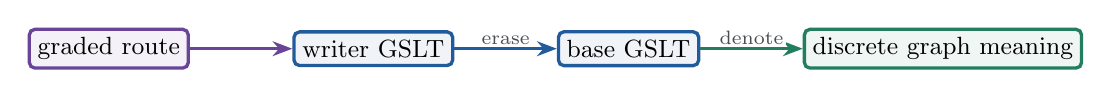
\begin{tikzpicture}[node distance=13mm]
  \node[cost,inner sep=3pt] (a) {graded route};
  \node[op,right=of a,inner sep=3pt] (b) {writer GSLT};
  \node[op,right=of b,inner sep=3pt] (c) {base GSLT};
  \node[math,right=of c,inner sep=3pt] (d) {discrete graph meaning};
  \draw[costflow] (a)--(b);
  \draw[opflow] (b)--node[lab,above]{erase}(c);
  \draw[semflow] (c)--node[lab,above]{denote}(d);
\end{tikzpicture}
}
\end{center}
The same graph can carry different resource accounts, so resources cannot be
reconstructed from graph meaning.

The detailed edge-list materializer supplies the first conversion grade with a
direct operational basis: a path contains one local write rewrite per stored
occurrence plus one finish rewrite.  Translating these structural events into
memory traffic or elapsed time still requires a separately justified physical
model.  For the remaining refinement legs, the present grades should be read
as explicit abstract assumptions used in break-even algebra, not as costs
extracted from hidden implementations.

\subsection{When is migration worth paying for?}

Suppose a source query costs \(t+s\), a target query costs \(t\), conversion
costs \(c\), and the future workload has \(q\) queries.  Exact arithmetic gives
\begin{theorem}[Static break-even]
\[
  c+qt<q(t+s)\quad\longleftrightarrow\quad c<qs.
\]
\end{theorem}
No asymptotic hand-waving is required.  Weighted finite workloads similarly
support exact average-case numerators, and pointwise dominance implies
dominance for every such weighted workload.

If both representations are retained as a coherent channel and each of \(e\)
edits costs an extra target synchronization \(u\), then:
\begin{theorem}[Dynamic multi-view break-even]
\[
  \text{maintain the second view faster}
  \quad\longleftrightarrow\quad
  c+eu<qs.
\]
\end{theorem}
Without query savings, every genuinely costly channel is slower.  A
time-winning channel may still be inadmissible because its two retained
carriers exceed the space budget.

\begin{figure}[htbp]
\centering
\resizebox{.95\textwidth}{!}{%
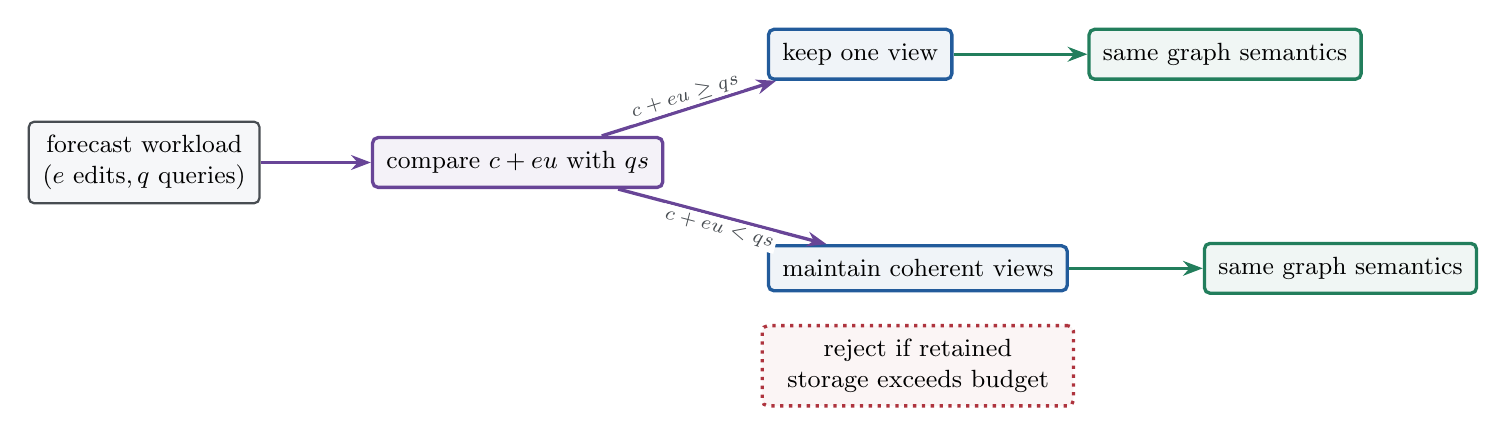
\begin{tikzpicture}[node distance=8mm and 14mm]
  \node[syntax] (work) {forecast workload\\\((e\ \text{edits},q\ \text{queries})\)};
  \node[cost,right=of work] (equation) {
    compare \(c+eu\) with \(qs\)};
  \node[op,above right=7mm and 13mm of equation] (single) {keep one view};
  \node[op,below right=7mm and 13mm of equation] (channel) {maintain coherent views};
  \node[math,right=17mm of single] (same1) {same graph semantics};
  \node[math,right=17mm of channel] (same2) {same graph semantics};
  \draw[costflow] (work)--(equation);
  \draw[costflow] (equation)--node[lab,above,sloped]{\(c+eu\ge qs\)}(single);
  \draw[costflow] (equation)--node[lab,below,sloped]{\(c+eu<qs\)}(channel);
  \draw[semflow] (single)--(same1);
  \draw[semflow] (channel)--(same2);
  \node[negative,below=4mm of channel,text width=36mm] (budget) {
    reject if retained storage exceeds budget};
\end{tikzpicture}}
\caption{Representation choice is a resource policy over already proved
semantic alternatives.  The policy may select a faster view; it cannot decide
whether an edge exists.}
\label{fig:break-even}
\end{figure}

This is the formal analogue of the representation portfolios and channelling
constraints used by Essence and Conjure \cite{essence,conjure}.  The difference
is that the representation maps and semantic coherence laws are checked, while
the cost policy remains explicitly separate from truth.

\subsection{Worked representation decisions}
\label{sec:worked-migration}

Constraint modelling makes the workload dependence concrete.  Essence lets a
problem be stated over an abstract combinatorial object; Conjure refines such
objects and expressions through representation choices, and can retain
multiple channelled representations \cite{essence,conjure}.  Our graph
examples isolate the corresponding decision after semantic correctness has
already been proved.  The unit below is a \emph{structural event}, not a timing
measurement: one edge occurrence consumed, one edge-list occurrence probed,
one matrix cell read, or one synchronized occurrence update.

\paragraph{Pairwise graph-isomorphism constraints: migrate.}
Consider one side of a graph-isomorphism model that ranges over every
unordered vertex pair and constrains whether adjacency is preserved by the
candidate bijection.  A 200-vertex simple graph with 800 distinct edges has
\(\binom{200}{2}-800=19{,}100\) absent pairs.  Those absent probes alone force
19,100 complete scans of an 800-occurrence edge list.  The detailed
materializer costs \(800+1=801\) rewrites and the matrix then costs one read per
probe:
\[
\begin{array}{rcl}
\mathsf{stay} &=& 19{,}100\cdot800=15{,}280{,}000,\\
\mathsf{migrate} &=& 801+19{,}100\cdot1=19{,}901.
\end{array}
\]
The Lean theorem proves the strict inequality.  Present-edge probes can only
add further nonnegative savings relative to this absent-pair subworkload, so
the decision does not depend on optimistic early matches.

\paragraph{Edge-driven graph colouring: do not migrate.}
In the standard colouring model, one inequality is emitted per authored edge:
\begin{lstlisting}[style=graphlang,language={}]
forAll (u,v) in edges(G) . colour[u] != colour[v]
\end{lstlisting}
Streaming the 800 edge occurrences costs 800 events.  Materializing the
matrix and using the selected full scan schedule over its \(200^2\) ordered
cells costs
\(801+40{,}000=40{,}801\).  Here the edge list already presents exactly the
iteration domain required by the constraints.  The negative theorem is as
important as the positive one: a matrix is not intrinsically the ``better''
representation.

\paragraph{A revised sparse graph: forecast both edits and reads.}
For a 1,000-vertex, 3,000-occurrence graph, initial materialization costs
3,001 events, the edge list occupies 6,000 endpoint cells, and the matrix
occupies 1,000,000 Boolean cells.  With 25 edits and ten absent-edge queries,
selecting one event for both the source update and target synchronization, the exact
accounts are
\[
  \mathsf{channelled}=3{,}001+25(1+1)+10=3{,}061,
  \qquad
  \mathsf{single}=25+10\cdot3{,}000=30{,}025.
\]
The maintained matrix wins on events.  With 4,000 edits and one query, the
ruling reverses:
\[
  \mathsf{single}=7{,}000 < 11{,}002=\mathsf{channelled}.
\]
Finally, even the read-heavy winner is inadmissible under a 750,000-cell
budget because retaining both views requires 1,006,000 cells.  All three
claims are checked concrete instances of the general break-even and space
laws, not prose estimates.  The unit edit and synchronization grades are
explicit model choices; unlike construction and query counts, they are not yet
extracted from a detailed edit implementation.

\begin{table}[htbp]
\centering
\small
\renewcommand{\arraystretch}{1.15}
\begin{tabularx}{\textwidth}{@{}Yrrl@{}}
\toprule
Workload & Source-only events & Alternative events & Ruling\\
\midrule
19,100 absent-pair probes & 15,280,000 & 19,901 & materialize matrix\\
edge-driven colouring & 800 & 40,801 & stream edge list\\
25 edits, 10 absent probes & 30,025 & 3,061 & maintain both views\\
4,000 edits, 1 absent probe & 7,000 & 11,002 & keep edge list\\
read-heavy, 750,000-cell budget & 6,000 retained & 1,006,000 retained & reject channel\\
\bottomrule
\end{tabularx}
\caption{Worked decisions in the selected structural-event model.  The same
semantically correct representations produce different optima because the
constraint iteration domain, revision rate, query rate, and storage budget
differ.}
\label{tab:worked-migration}
\end{table}

\section{Higher graphs and controlled information loss}
\label{sec:higher}

Ordinary simple graphs are only one semantic level.  The same method is
applied to three richer structures.

\subsection{Hypergraphs}

A finite hypergraph stores named edge occurrences with finite vertex supports
\cite{berge}.
The incidence query has a detailed linear-scan GSLT and an exact semantic
query translation.  Two standard projections are formalized as total maps:
\begin{itemize}[leftmargin=2em]
  \item the \emph{two-section}, connecting two vertices when some hyperedge
        contains both;
  \item the bipartite \emph{Levi graph}, connecting vertex objects to edge
        objects by incidence.
\end{itemize}
The existing one-step Levi transition records application of the projection,
but does not yet expose an occurrence-by-occurrence Levi construction.  It is
therefore classified here as an abstract refinement leg.  A sharp negative
example shows that one ternary hyperedge and three binary hyperedges can have
the same two-section while retaining different hyperedge-occurrence counts.
Hence the two-section preserves pairwise adjacency but cannot reconstruct
grouping or occurrence identity.

\subsection{Enriched metagraphs}

The metagraph carrier gives each object an authored list of ports.  A port has
a target, label, and enrichment payload.  Link querying is executable and
proved against the corresponding relational meaning.  Forgetting to an
underlying hypergraph preserves selected incidence but loses port order,
labels, and enrichment.  Reordered authored ports therefore provide a
negative witness: the underlying relational worlds agree while the metagraph
worlds remain distinct.

\subsection{Distinction graphs}

A finite sampled distinction structure is mapped to an adjacency matrix.
The refinement theorem characterizes every cell, and its abstract transition
composes with matrix querying and semantic Boolean answering.  A detailed
row/cell construction machine remains work in progress.  The source sample is
retained in the state because a matrix records that a separator exists, not
which semantic witness established it.  Two witnessed tables can erase to the
same matrix with different witnesses; no global inverse is claimed.

\begin{figure}[htbp]
\centering
\resizebox{.96\textwidth}{!}{%
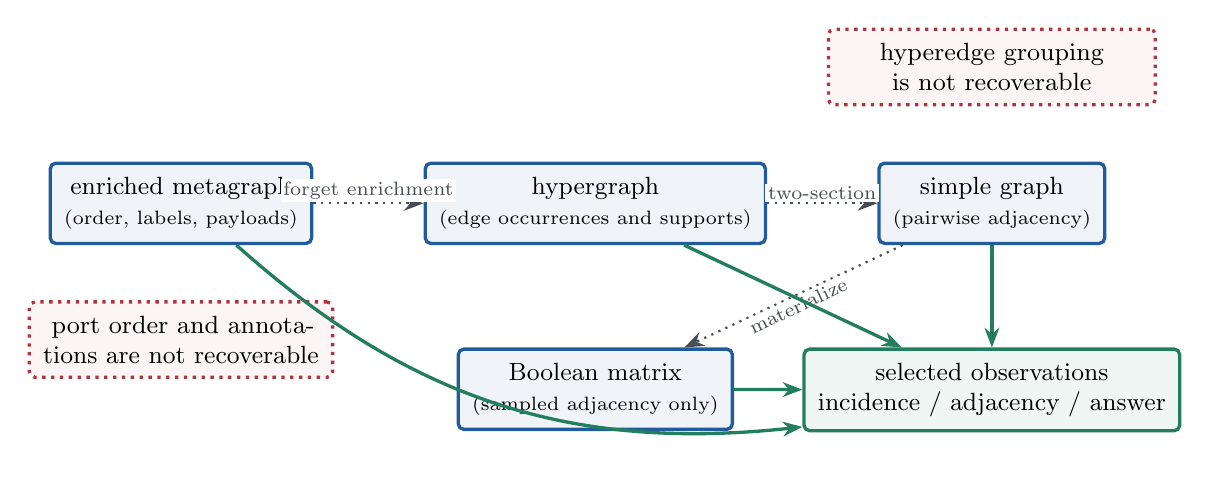
\begin{tikzpicture}[node distance=10mm and 14mm]
  \node[op] (meta) {enriched metagraph\\
    \scriptsize(order, labels, payloads)};
  \node[op,right=of meta] (hyper) {hypergraph\\
    \scriptsize(edge occurrences and supports)};
  \node[op,right=of hyper] (simple) {simple graph\\
    \scriptsize(pairwise adjacency)};
  \node[op,below=13mm of hyper] (matrix) {Boolean matrix\\
    \scriptsize(sampled adjacency only)};

  \draw[forgetflow] (meta)--node[lab,above]{forget enrichment}(hyper);
  \draw[forgetflow] (hyper)--node[lab,above]{two-section}(simple);
  \draw[forgetflow] (simple)--node[lab,below,sloped]{materialize}(matrix);

  \node[negative,below=7mm of meta,text width=35mm] {
    port order and annotations are not recoverable};
  \node[negative,above=7mm of simple,text width=38mm] {
    hyperedge grouping is not recoverable};
  \node[negative,right=11mm of matrix,text width=37mm] {
    distinction witness is not recoverable};

  \node[math,below=13mm of simple] (obs) {selected observations\\
    incidence / adjacency / answer};
  \draw[semflow] (meta) to[bend right=24] (obs);
  \draw[semflow] (hyper) -- (obs);
  \draw[semflow] (simple) -- (obs);
  \draw[semflow] (matrix) -- (obs);
\end{tikzpicture}}
\caption{A hierarchy of useful forgetful maps.  Each arrow preserves a named
observation and has a negative theorem showing which richer structure is
lost.  Semantic adequacy is not misreported as representational invertibility.}
\label{fig:higher-loss}
\end{figure}

Rotation systems fit the same picture: a cyclic order around each vertex is
an enrichment of adjacency, not another lossless encoding of a plain graph.

\section{Transporting ordinary graph theorems}
\label{sec:theorem-transport}

Since every abstract refinement path preserves the exact Mathlib graph,
\emph{every}
predicate on finite simple graphs transports.  For
\[
  P : \SG(\Fin n)\longrightarrow\Prop,
\]
the generic result is
\[
  P(\denote{s})
  \quad\longleftrightarrow\quad
  P(\denote{\mathsf{convert}(s,L)}).
\]
Specialized corollaries cover connectedness, bipartiteness, acyclicity,
Hamiltonicity, and neighbour-set cardinality.  Cost is deliberately absent:
an absent edge in the path edge list takes two probes but one after matrix
materialization, even though every extensional graph theorem is preserved.

\subsection{Hamiltonian cycles, Ore, and Dirac}

The declarative graph library contains a custom finite Hamilton-cycle
certificate with an exact bridge to Mathlib's walk-based
\(\mathsf{IsHamiltonianCycle}\): the constructed walk has the expected length,
the expected vertex at each index, and visits every vertex in the required
cyclic order.

Ore's theorem is proved by the standard longest-path rotation argument
\cite{ore,diestel}.  For \(|V|\ge3\), if every distinct nonadjacent pair
satisfies
\[
  |V|\le \deg(u)+\deg(v),
\]
then the graph is Hamiltonian.  Dirac's theorem is derived as the specialization
\(|V|\le2\delta(G)\) \cite{dirac}.  The two operational transport theorems say:
if the degree premise holds for the graph denoted by \emph{any} source layout,
then every materialized target layout denotes a Hamiltonian graph.

\begin{figure}[htbp]
\centering
\resizebox{.96\textwidth}{!}{%
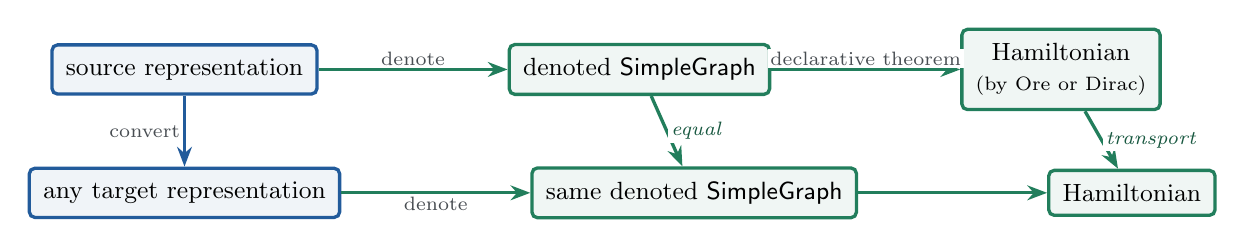
\begin{tikzpicture}[node distance=9mm and 24mm]
  \node[op] (src) {source representation};
  \node[math,right=of src] (g) {denoted \(\SG\)};
  \node[math,right=of g] (ham) {Hamiltonian\\
    \scriptsize(by Ore or Dirac)};
  \node[op,below=of src] (dst) {any target representation};
  \node[math,right=of dst] (gd) {same denoted \(\SG\)};
  \node[math,right=of gd] (hamd) {Hamiltonian};
  \draw[semflow] (src)--node[lab,above]{denote}(g);
  \draw[semflow] (g)--node[lab,above]{declarative theorem}(ham);
  \draw[opflow] (src)--node[lab,left]{convert}(dst);
  \draw[semflow] (dst)--node[lab,below]{denote}(gd);
  \draw[semflow] (g)--node[thmlab,right]{equal}(gd);
  \draw[semflow] (ham)--node[thmlab,right]{transport}(hamd);
  \draw[semflow] (gd)--(hamd);
\end{tikzpicture}
}
\caption{A declarative theorem is proved once over the standard graph and
then transported through every representation refinement.  This
is property transport, not a claim that the conversion finds a Hamiltonian
cycle efficiently.}
\label{fig:hamilton-transport}
\end{figure}

The Chv\'atal--Erd\H{o}s theorem is not part of the current formalization.  An
earlier unproved declaration was removed.  A real proof requires a canonical
separator/connectivity interface, a Menger-style bridge, and a longest-cycle
argument; retaining the gap explicitly is more informative than preserving a
name without a theorem.

\clearpage
\section{When a LanguageDef has transformation semantics}
\label{sec:vocabulary}

An earlier draft included a validated \code{LanguageDef} that declared names
for graphs, layouts, routes, plans, and commands while providing no equations
or rewrites.  That declaration has been removed from the active graph
umbrella and from the claimed formal stack.  Validation of a constructor
vocabulary establishes only that the declaration is internally well formed;
it does not determine graph payloads, route endpoints, conversion behavior,
or execution.

The negative criterion is simple.  If two incompatible conversion functions
can be placed behind the same declared route name without changing the
\code{LanguageDef}, then the declaration is not an authority for that
conversion.  Similarly, a term such as \code{via(plan, graph)} has no
operational content until its graph encoding, typed plan elaboration, and
rewrite behavior are derived from inspectable rules.

Sections~\ref{sec:matrix-langdef} and~\ref{sec:walk-langdef} supply two
positive replacements.  The first encodes a complete conversion state, lets
two rewrites determine every successor, and commutes with an independent
matrix interpretation.  The second gives thirteen local rules for three
ordinary walk operations and proves exact correspondence with Mathlib.  Both
are genuine operational language definitions; neither delegates its complete
operation to an external relation.

Section~\ref{sec:walk-ntt} adds a second test: a useful LanguageDef should
support derived judgments that actually depend on its syntax and dynamics.
The walk native type depends simultaneously on generated sort checking,
constructor fibres, and successful guarded execution.  Removing the adjacency
premise changes the negative theorem, and changing the rewrite table changes
the behavioral modality.  The type theory is therefore downstream of the
LanguageDef rather than administrative metadata placed beside it.

It is not yet a general graph-plan language.  Such a language still needs a
canonical graph payload codec, endpoint-safe typed plan elaboration, local
rules for every supported algorithm, and a generated runtime realization.
Plan composition may then elaborate into the existing indexed path category.
That broader contract is stated in Appendix~\ref{app:frontend}; the selected
materializer is its first proved vertical, not evidence that every abstract
route already has detailed syntax and execution.

\section{Why this organization scales beyond graphs}
\label{sec:logic}

The same distinction applies to terms, formulas, proof states, and cognitive
world models.  A term may be represented as a tree, a DAG with shared
subterms, an e-graph, a hash-consed heap, or a serialized array.  These can
denote the same syntax while having very different substitution, revision,
sharing, and query costs.  Rewriting the representation is semantically silent
only relative to a selected meaning; beta reduction or belief revision changes
that meaning and needs a semantic step.

The graph development therefore suggests a reusable recipe:
\begin{enumerate}[label=\arabic*.,leftmargin=2.2em]
  \item choose an established declarative object;
  \item define concrete presentations and independent denotations;
  \item make each conversion an actual refinement;
  \item expose execution as a proof-relevant GSLT;
  \item map conversion to discrete semantics, revision to semantic dynamics,
        and queries to semantic request/answer machines;
  \item add cost only as selected grading over exposed local steps, or label it
        explicitly as an abstract model over refinement legs;
  \item prove both a useful positive result and a discriminating negative
        result for every abstraction boundary.
\end{enumerate}
For world-model calculi, this says that one world may have many physical
representations, each with distinct revision and extraction behavior.  A
planner over Bayesian networks or a probabilistic logic engine over decision
diagrams can then be studied as a representation-sensitive coGSLT-like
interface without turning scheduling, probability tables, or cache layout into
semantic truth.

\section{Formal inventory and theorem map}
\label{sec:inventory}

Table~\ref{tab:modules} lists the principal formal components.  Module names
are given rather than unstable line numbers.

\begin{table}[htbp]
\centering
\footnotesize
\renewcommand{\arraystretch}{1.13}
\begin{tabularx}{\textwidth}{@{}p{.34\textwidth}X@{}}
\toprule
Module family & Principal checked content \\
\midrule
\code{Representation.Basic} & Presentation, refinement, category, channel,
measured linear-probe GSLT.\\
\code{EdgeList}, \code{AdjacencyMatrix}, \code{AdjacencyRows},
\code{NeighborFinsets}, \code{IncidenceMatrix}, \code{CSR} & Six concrete
carriers, independent denotations, sound edge observers, storage/work facts,
positive and negative controls.\\
\code{Transformations}, \code{RepresentationGSLT} & Actual conversion maps,
ten abstract refinement legs, path composition, total routes through the
matrix waist, and adjacency no-invention.\\
\code{EdgeListToMatrixGSLT} & Occurrence-by-occurrence symmetric cell updates,
executable/relational step equivalence, exact completion invariant,
\(m+1\)-step path, exact equality with the matrix refinement, and positive and
negative controls.\\
\code{EdgeListToMatrixLanguageDef} & Five sorts, nine sorted constructors,
two operational rewrite rows, exact generic-executor/typed-step agreement,
terminal rejection, a commuting interpretation into the detailed matrix
machine, and exact endpoint denotation.\\
\code{GraphTheory.Walk.LanguageDef},
\code{GraphTheory.Walk.Operational},
\code{GraphTheory.Walk.Examples} & Five sorts, sixteen sorted constructors,
thirteen recursive rewrite rows, exact append/reverse/map executions to
Mathlib walks, closed path-length formulas, and endpoint-mismatch/non-edge
rejection controls.\\
\code{OSLF.Framework.PathTypeSynthesis},
\code{OSLF.MeTTaIL.NonrecursiveReduction} & Generic proof-relevant finite-path
and exact-length modalities, their Galois connections, path decomposition,
and exact one-layer execution for congruence-free LanguageDefs.\\
\code{GraphTheory.Walk.NativeTypeTheory},
\code{GraphTheory.Walk.ProofTheory},
\code{GraphTheory.Walk.NativeTypeExamples} & Generated static/dynamic native
walk judgment, canonical Mathlib inhabitation, injective encoding, exact-work
behavioral types, reachability category/groupoid operations, functorial map,
and endpoint/non-edge native-type controls.\\
\code{GSLT.Core.SemanticInvariant}, \code{SemanticTransport} & Invariants,
semantic fibres, equivalence with discrete realizations, denotation squares,
composition and path commutation.\\
\code{SemanticRevisionGSLT}, \code{RevisionQuery},
\code{RevisionPortfolio}, \code{WorldModelGSLT} & Independent semantic query
and revision dynamics, concrete translation, covered reflection, full
execution agreement, editable portfolio and world-model extraction.\\
\code{MatrixBridge} & Exact image in ordinary Boolean matrices, round trip,
injectivity, adjacency/cell theorem, answer-blind matrix query simulation and
reflection.\\
\code{CostModel}, \code{GSLT.Core.CostedOperational},
\code{CostedRepresentationGSLT}, \code{MultiView},
\code{MigrationExamples} & Resource monoid,
in-place/persistent envelopes, exact break-even laws, costed-theory category,
writer functor, natural erasure, proof-relevant graded routes, channel costs,
and worked positive/negative workload decisions.\\
\code{Hypergraph}, \code{Metagraph}, \code{DistinctionBridge},
\code{HigherGraphSemanticGSLT}, \code{RotationSystem} & Higher-graph
transformations and semantic queries, plus explicit information-loss
counterexamples.\\
\code{Hamiltonicity}, \code{HamiltonianDegree},
\code{Representation.SemanticTransport} & Hamilton-cycle/Mathlib bridge,
longest-path proof of Ore and Dirac, and property transport through every
layout.\\
\bottomrule
\end{tabularx}
\caption{The formal stack.  Declarative mathematics, operational rules,
semantic interpretation, and resource grading occupy different modules and
are connected by named theorems.}
\label{tab:modules}
\end{table}

At the formalization snapshot described here, the graph-representation umbrella
builds successfully with the operational matrix-construction and walk
\code{LanguageDef}s included and the earlier empty graph vocabulary excluded.
Focused audits of this tranche
find no proof placeholders, theorem wishlists, native-decision shortcuts, or
new project axioms.  Axiom reports for the selected theorems remain within
ordinary Lean foundations where required (propositional extensionality,
classical choice, and quotient soundness).  These facts concern the Lean
objects above; they do not certify an as-yet-unwritten CeTTa runtime or solver
connection.

\section{Conclusion}

The useful abstraction is not ``the adjacency matrix is the graph'' and not
``all representations are interchangeable.''  It is a network of concrete
presentations over a shared mathematical object, with proof-bearing
constructions between them and explicit operational theories for the motions
that matter.

In the resulting picture:
\begin{itemize}[leftmargin=2em]
  \item Mathlib graph theory says what a graph and its properties mean;
  \item refinement functions say which target carriers are constructed and
        prove what those carriers denote;
  \item detailed GSLTs say how exposed local states transform;
  \item native types organize constructor shape, endpoint fibres, and
        behavioral reachability into derived mathematical judgments;
  \item semantic revision and query GSLTs say how graph meaning and
        observations evolve;
  \item operational realizations and denotation squares make the entire chain
        compose;
  \item costed theories say when a correct representation change is worth its
        time and space;
  \item negative theorems say exactly what every forgetful map loses.
\end{itemize}
That organization is useful for ordinary graph algorithms, but its larger
value is methodological.  It offers a prototype mathematical library in which
declarative truth and operational behavior are both first-class, cleanly
separated, and then reconnected by proofs.

\appendix

\section{Work in progress: detailed transformation portfolio}
\label{app:detailed-portfolio}

The edge-list materializer is the first detailed conversion, not evidence that
the remaining refinement legs are already small-step algorithms.  The next
three machines form the most informative end-to-end chain:
\begin{enumerate}[label=\arabic*.,leftmargin=2.2em]
  \item \textbf{Matrix to adjacency rows.}  Scan coordinates in canonical
        row-major order, append a target exactly when the matrix cell is true,
        retain the current row and completed rows, and prove exact terminal
        equality with \code{matrixToRows}.  The loop invariant must identify
        the accumulator with the processed prefix of coordinates.
  \item \textbf{Adjacency rows to CSR.}  Consume one row item at a time,
        maintain offsets and payload, prove monotone and bounded offsets, and
        prove exact equality with \code{rowsToCSR}.  Prefix-sum and payload
        actions, rather than a hidden packing function, provide the cost basis.
  \item \textbf{Composed realization.}  Compose edge-list materialization,
        row expansion, and CSR packing while retaining every local event.
        Prove that erasure yields the existing three-leg refinement itinerary
        and that the final CSR carrier is exactly the existing total
        conversion result.
\end{enumerate}

Further detailed candidates include matrix-to-edge-list cell scanning,
matrix-to-incidence column construction, occurrence-preserving Levi graph
materialization, and row/cell construction for distinction matrices.  Until
their states, local rewrites, invariants, and endpoint theorems exist, their
current one-step transitions remain classified as abstract refinement legs.

\section{Work in progress: from walks to path rewriting}
\label{app:walk-rewriting}

The implemented walk machine deliberately stops at total append, reverse, and
homomorphic map.  These operations already expose recursion and relation
queries, and their generated native types already support the category laws,
involutive reversal, and functorial homomorphic map on canonical reachability
proofs.  They do not yet form a normalization theory of paths.  The next
mathematically substantive extension is the free-groupoid view of an
undirected graph: vertices are objects, walks are composable arrows, reversal
is inversion, and an immediately retraced edge may cancel.

A candidate local rule has the genuinely inspectable form
\[
  (u\!\to\!v);(v\!\to\!u);p \;\longrightarrow\; p,
\]
with both adjacencies and all endpoints explicit.  Before admitting that rule
to the solid language, the formalization must prove termination of the chosen
orientation, confluence or a characterized normal-form relation, compatibility
with append, and correspondence with the intended quotient of Mathlib walks.
It must also distinguish cancellation of immediate backtracking from the
stronger and generally false claim that arbitrary cycles disappear.

A separate exactness obligation remains for the present native type.  The
solid development proves that every Mathlib walk has an injective canonical
native encoding and supplies discriminating negative cases.  Full no-junk
requires inversion of arbitrary generated reversal paths to reconstruct a
dependent Mathlib walk from every accepted raw pattern.  That theorem must be
proved from the constructor checker, the guarded scan rows, and relation-query
exactness; it may not be obtained by adding a hidden host-language decoder to
the definition of \code{NativeWalk}.

Two further extensions should remain separate.  An incremental trail/path
admission machine can carry visited edge or vertex sets and reject the first
duplicate occurrence; this operationalizes Mathlib's \code{IsTrail} and
\code{IsPath} predicates without changing walk equality.  A reachability
search machine can nondeterministically extend a frontier one adjacent edge at
a time and return witness walks.  Search policy, fairness, and resource bounds
belong to that latter GSLT, not inside an opaque \code{reachable} relation.
The already-proved functorial laws for canonical native proofs should then be
strengthened from equality of their Mathlib witnesses to commuting diagrams
between the retained map executions themselves.

\section{Work in progress: general source language and compiler}
\label{app:frontend}

The selected edge-list materializer now establishes a narrow but complete
source-language vertical: sorted constructors and two rewrites drive the
generic executor, exact successor agreement connects it to a typed action
function, and independent denotation connects that action to the detailed
matrix machine.  The remaining goal is to generalize this result to graph
payload parsing, multiple conversion algorithms, and typed plan composition.
That broader minimum vertical is:
\begin{center}
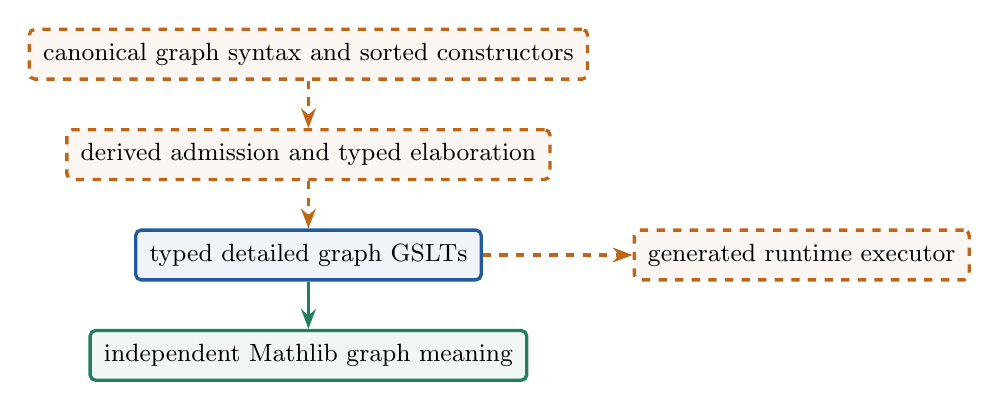
\begin{tikzpicture}[node distance=6mm]
  \node[future] (syntax) {canonical graph syntax and sorted constructors};
  \node[future,below=of syntax] (elab) {derived admission and typed elaboration};
  \node[op,below=of elab] (typed) {typed detailed graph GSLTs};
  \node[math,below=of typed] (meaning) {independent Mathlib graph meaning};
  \node[future,right=19mm of typed] (runtime) {generated runtime executor};
  \draw[futureflow] (syntax)--(elab);
  \draw[futureflow] (elab)--(typed);
  \draw[semflow] (typed)--(meaning);
  \draw[futureflow] (typed)--(runtime);
\end{tikzpicture}
\end{center}
Remaining theorems include canonical text/payload codec round trips,
exact-image characterization, admission soundness and reflection,
endpoint-safe plan composition, equality between elaborated plans and indexed
GSLT paths, and a source-to-runtime operational realization.  The current
persistent update node must additionally be refined into address calculation
and concrete cell writes before any row-major physical-cost claim.  A
validated vocabulary with empty rewrites satisfies none of these obligations.

\section{Work in progress: cost, editing, and certified solving}
\label{app:later}

The detailed machines should next support local, persistent, and differential
edit algorithms as competing refinements.  Their structural event grades must
then be related to selected physical implementations before making hardware
or elapsed-time claims.  Mixed revision/query workloads and maintained
multi-view channels require the same treatment.

For finite-search graph properties, the intended architecture is a proved
refinement into a standard solver boundary:
\begin{center}
\resizebox{\textwidth}{!}{%
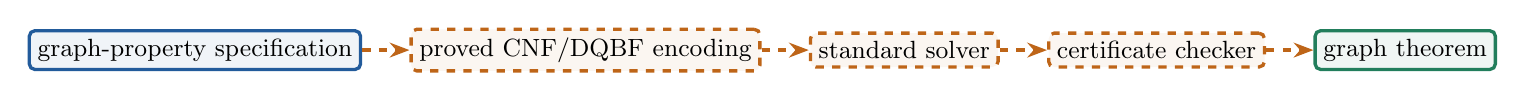
\begin{tikzpicture}[baseline=-1mm,node distance=6mm]
  \node[op,inner sep=3pt] (problem) {graph-property specification};
  \node[future,right=of problem,inner sep=3pt] (cnf) {proved CNF/DQBF encoding};
  \node[future,right=of cnf,inner sep=3pt] (solve) {standard solver};
  \node[future,right=of solve,inner sep=3pt] (cert) {certificate checker};
  \node[math,right=of cert,inner sep=3pt] (claim) {graph theorem};
  \draw[futureflow] (problem)--(cnf);
  \draw[futureflow] (cnf)--(solve);
  \draw[futureflow] (solve)--(cert);
  \draw[futureflow] (cert)--(claim);
\end{tikzpicture}}
\end{center}
The solver may be untrusted; the encoding theorem and certificate replay are
the trusted arrows.  This boundary is not yet connected to the graph GSLTs and
is not part of the proved vertical.

The remaining research programme is:
\begin{enumerate}[label=\arabic*.,leftmargin=2.2em]
  \item complete and compose the detailed matrix-to-rows and rows-to-CSR
        machines;
  \item prove raw-pattern no-junk for \code{NativeWalk}, then add terminating
        and confluent immediate-backtrack cancellation plus incremental
        trail/path admission;
  \item generalize the selected operational \code{LanguageDef} into a
        canonical graph-payload codec and endpoint-safe typed plan compiler;
  \item connect structural grades to selected physical implementations and
        measurements;
  \item extend higher graphs from detailed queries to occurrence-preserving
        revision and construction machines;
  \item connect graph-property specifications to certified
        SAT/DQBF/SMT/ILP encodings and replayed certificates;
  \item formalize Chv\'atal--Erd\H{o}s from separator, Menger, and
        longest-cycle infrastructure;
  \item realize a selected workload in CeTTa and prove the complete
        source--semantic--runtime commuting diagram, including severance
        gates.
\end{enumerate}

Two dangers dominate this programme.  Equality of denotation must not be
inflated into recovery of erased order, occurrence, provenance, witnesses, or
cost.  And a generated target must be the output of an actual lowering
function with a commuting theorem; agreement with a separately handwritten
implementation is valuable differential evidence, but it is not generation.

\begin{thebibliography}{99}

\bibitem{mathlib}
The Mathlib Community.
\newblock The Lean Mathematical Library.
\newblock In \emph{Proceedings of CPP 2020}, pages 367--381, 2020.
\newblock \href{https://doi.org/10.1145/3372885.3373824}{doi:10.1145/3372885.3373824}.

\bibitem{diestel}
Reinhard Diestel.
\newblock \emph{Graph Theory}, fifth edition.
\newblock Springer, 2017.
\newblock \href{https://doi.org/10.1007/978-3-662-53622-3}{doi:10.1007/978-3-662-53622-3}.

\bibitem{essence}
Alan M. Frisch, Warwick Harvey, Christopher Jefferson,
Bernadette Mart\'inez-Hern\'andez, and Ian Miguel.
\newblock Essence: A constraint language for specifying combinatorial problems.
\newblock \emph{Constraints}, 13:268--306, 2008.
\newblock \href{https://doi.org/10.1007/s10601-008-9047-y}{doi:10.1007/s10601-008-9047-y}.

\bibitem{conjure}
\c{C}a\u{g}da\c{s} Akg\"un, Alan M. Frisch, Ian P. Gent, Christopher Jefferson,
Ian Miguel, and Peter Nightingale.
\newblock Conjure: Automatic generation of constraint models from problem
specifications.
\newblock \emph{Artificial Intelligence}, 310:103751, 2022.
\newblock \href{https://doi.org/10.1016/j.artint.2022.103751}{doi:10.1016/j.artint.2022.103751}.

\bibitem{turi-plotkin}
Daniele Turi and Gordon Plotkin.
\newblock Towards a mathematical operational semantics.
\newblock In \emph{Proceedings of LICS 1997}, pages 280--291, 1997.
\newblock \href{https://doi.org/10.1109/LICS.1997.614955}{doi:10.1109/LICS.1997.614955}.

\bibitem{moggi}
Eugenio Moggi.
\newblock Notions of computation and monads.
\newblock \emph{Information and Computation}, 93(1):55--92, 1991.
\newblock \href{https://doi.org/10.1016/0890-5401(91)90052-4}{doi:10.1016/0890-5401(91)90052-4}.

\bibitem{berge}
Claude Berge.
\newblock \emph{Hypergraphs: Combinatorics of Finite Sets}.
\newblock North-Holland, 1989.

\bibitem{dirac}
G. A. Dirac.
\newblock Some theorems on abstract graphs.
\newblock \emph{Proceedings of the London Mathematical Society},
s3-2(1):69--81, 1952.
\newblock \href{https://doi.org/10.1112/plms/s3-2.1.69}{doi:10.1112/plms/s3-2.1.69}.

\bibitem{ore}
Oystein Ore.
\newblock Note on Hamilton circuits.
\newblock \emph{The American Mathematical Monthly}, 67(1):55, 1960.
\newblock \href{https://doi.org/10.2307/2308928}{doi:10.2307/2308928}.

\bibitem{meredith}
L. Gregory Meredith.
\newblock Computation, causality, and consciousness.
\newblock Manuscript, 2026.

\end{thebibliography}

\end{document}
